\documentclass[aspectratio=169,9pt]{beamer}

\usepackage{graphicx,caption,subcaption,hyperref,amsmath,tikz}
\graphicspath{ {./figures/} }
\captionsetup{font=scriptsize,labelfont=scriptsize}
\setbeamerfont{footnote}{size=\scriptsize}
\usepackage[strict]{changepage}
\usetikzlibrary{arrows,automata,positioning}
\usetheme[titleformat=smallcaps,
            sectionpage=progressbar,
			subsectionpage=progressbar,
			progressbar=frametitle,
			numbering=fraction]{metropolis}
% \usecolortheme{owl}
\usepackage[style=apa,
			sorting=nyt,
			date=year,
			bibencoding=utf8,
			isbn=false,
			eprint=false,
			dashed=false,
			uniquelist=false,
			maxbibnames=10,
			minbibnames=1,
			maxcitenames=2,
			uniquename=init,
			giveninits=true,
			useprefix=false,
			minsortnames=1,
			maxsortnames=2]{biblatex}
\bibliography{References}

% Information to be included in the title page:
\title{Modelling of X-Chromosome reactivation by Toggle switch}
\author{Harshavardhan BV}
\date{\today}
\institute{IISc Bangalore}

\begin{document}
    \frame{\titlepage}

    \section{Introduction}
    \begin{frame}{Origin of X-Chromosome inactivation \& upregulation}
        \begin{figure}
            \centering
            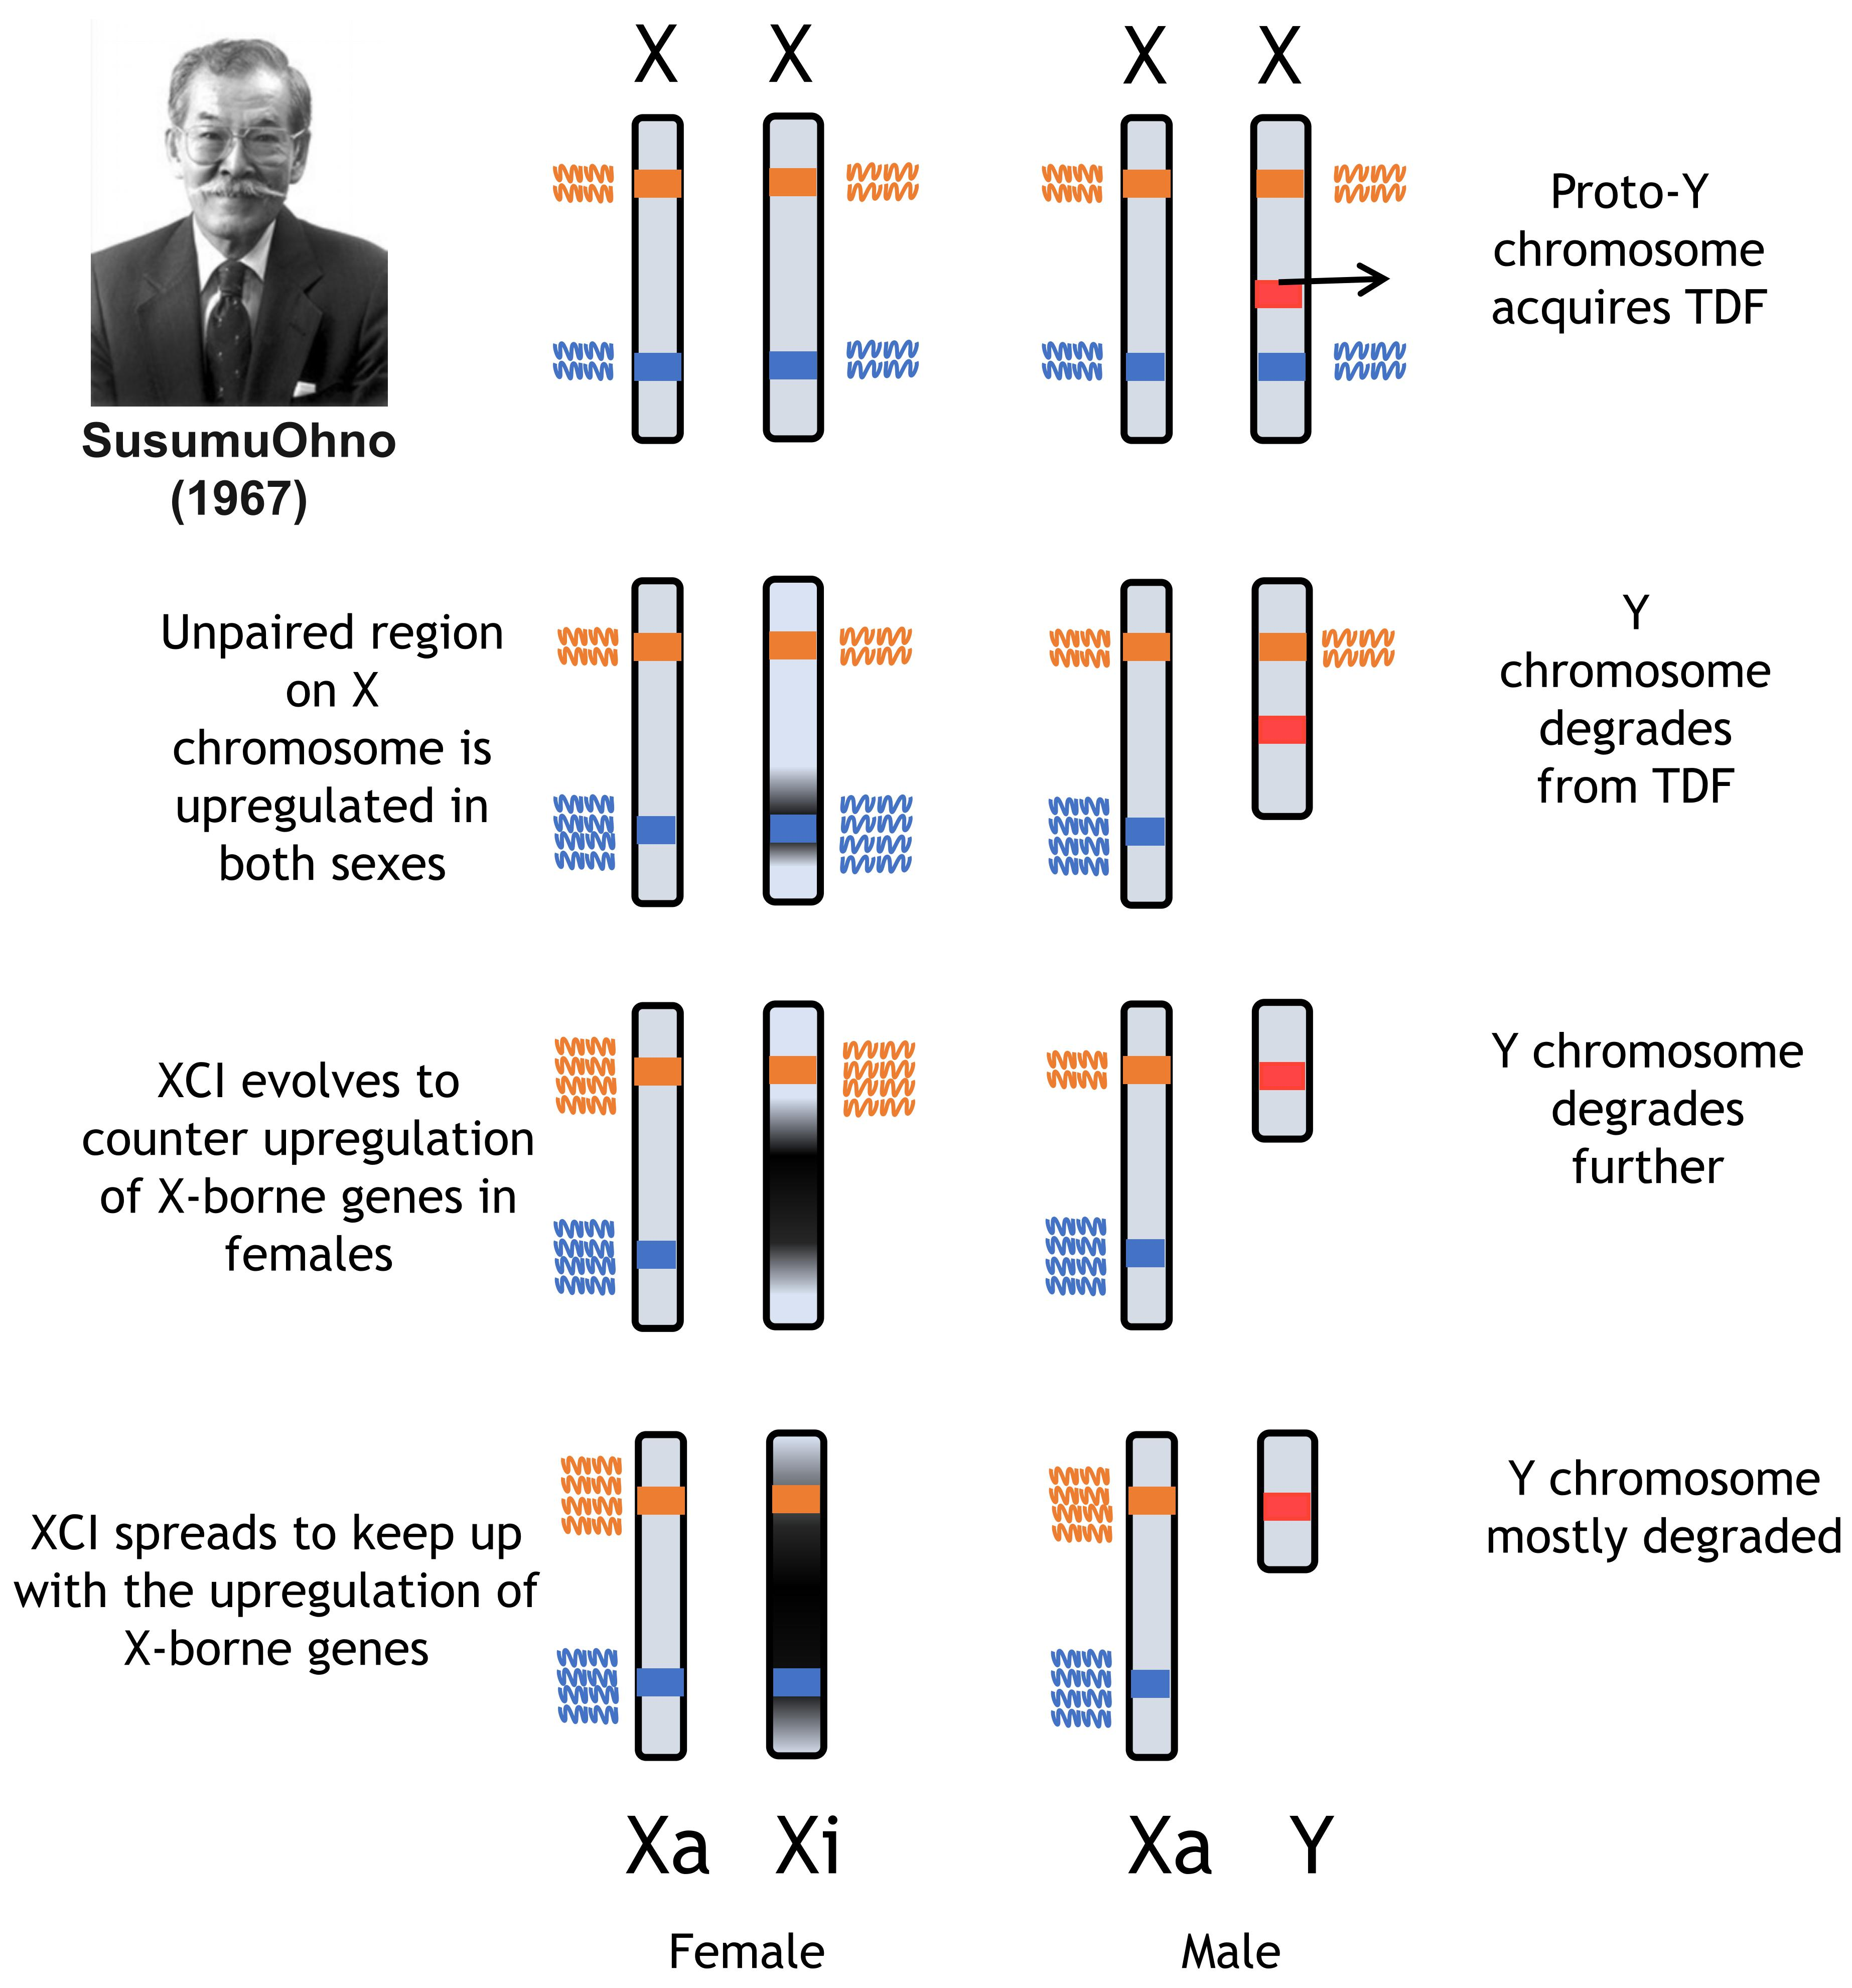
\includegraphics[width=0.42\textwidth]{ohno}
            \caption{Ohno's hypothesis for X-Chromosome upregulation \footcite{ohno} \footnote{Credits: Srimonta Gayen}}
        \end{figure}
    \end{frame}

    \begin{frame}{Mechanism of X-Chromosome upregulation}
        \begin{figure}
            \centering
            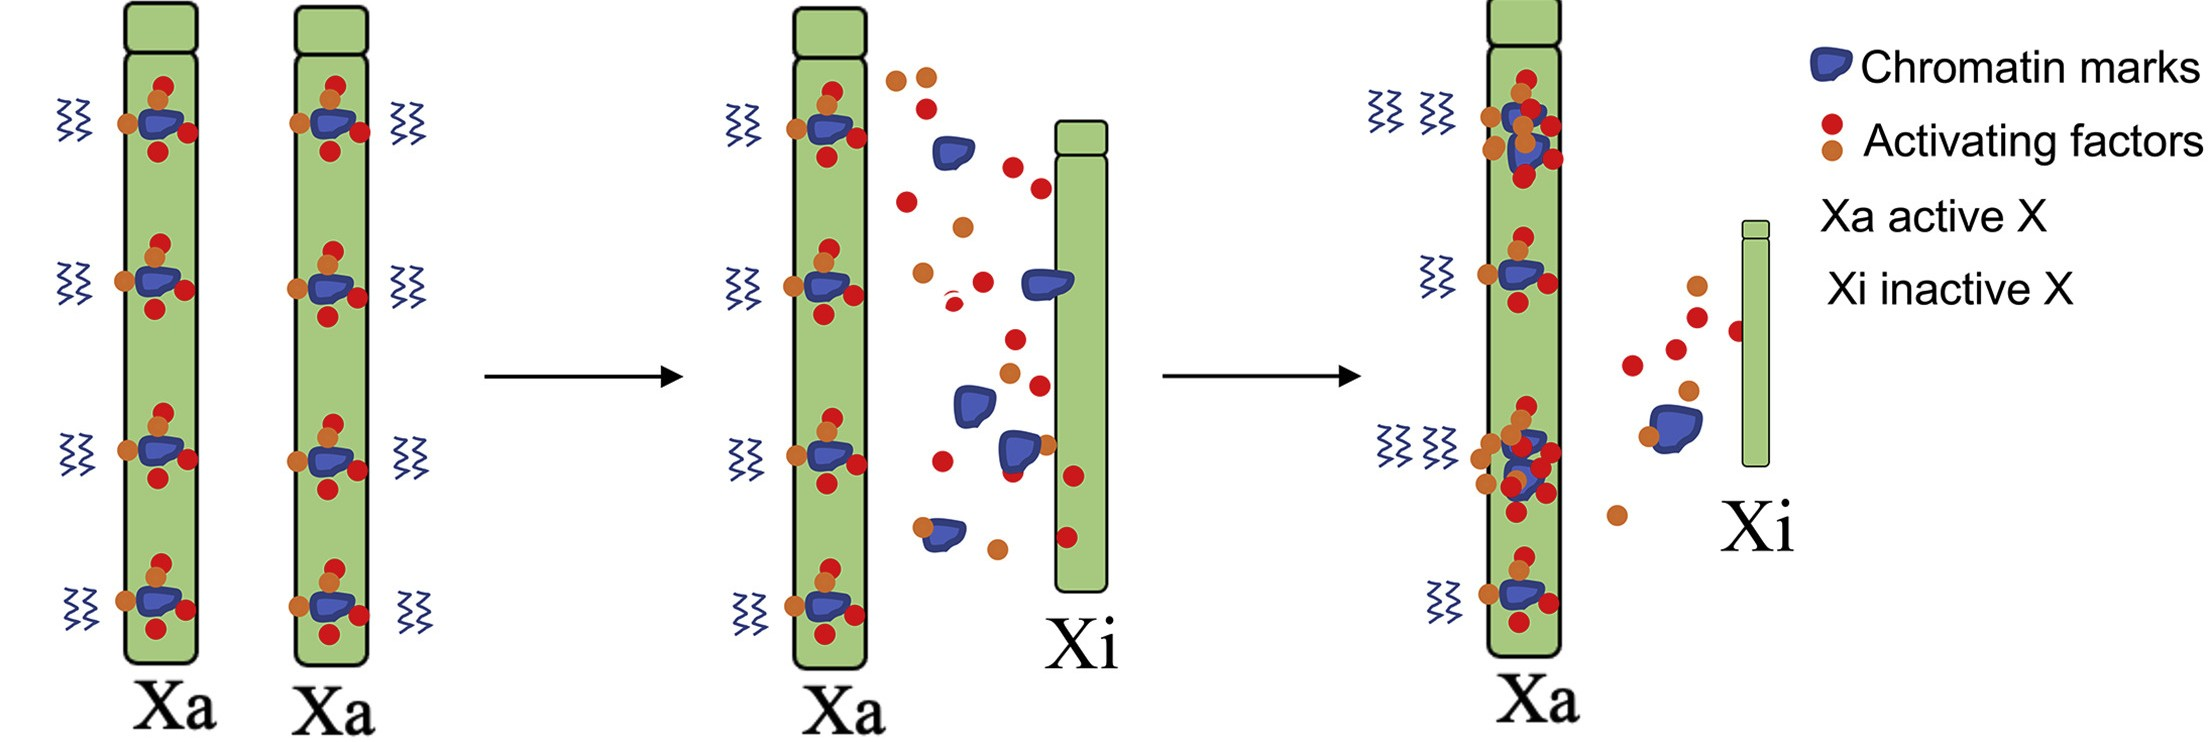
\includegraphics[width=0.7\textwidth]{xcu}
            \caption{Model describing a mechanism of X-Chromosome upregulation \footcite{XCI} \footnote{Credits: Kishore Hari}}
        \end{figure}
    \end{frame}

    \begin{frame}{Occurance of X-chromosome reactivation}
        \begin{figure}
            \centering
            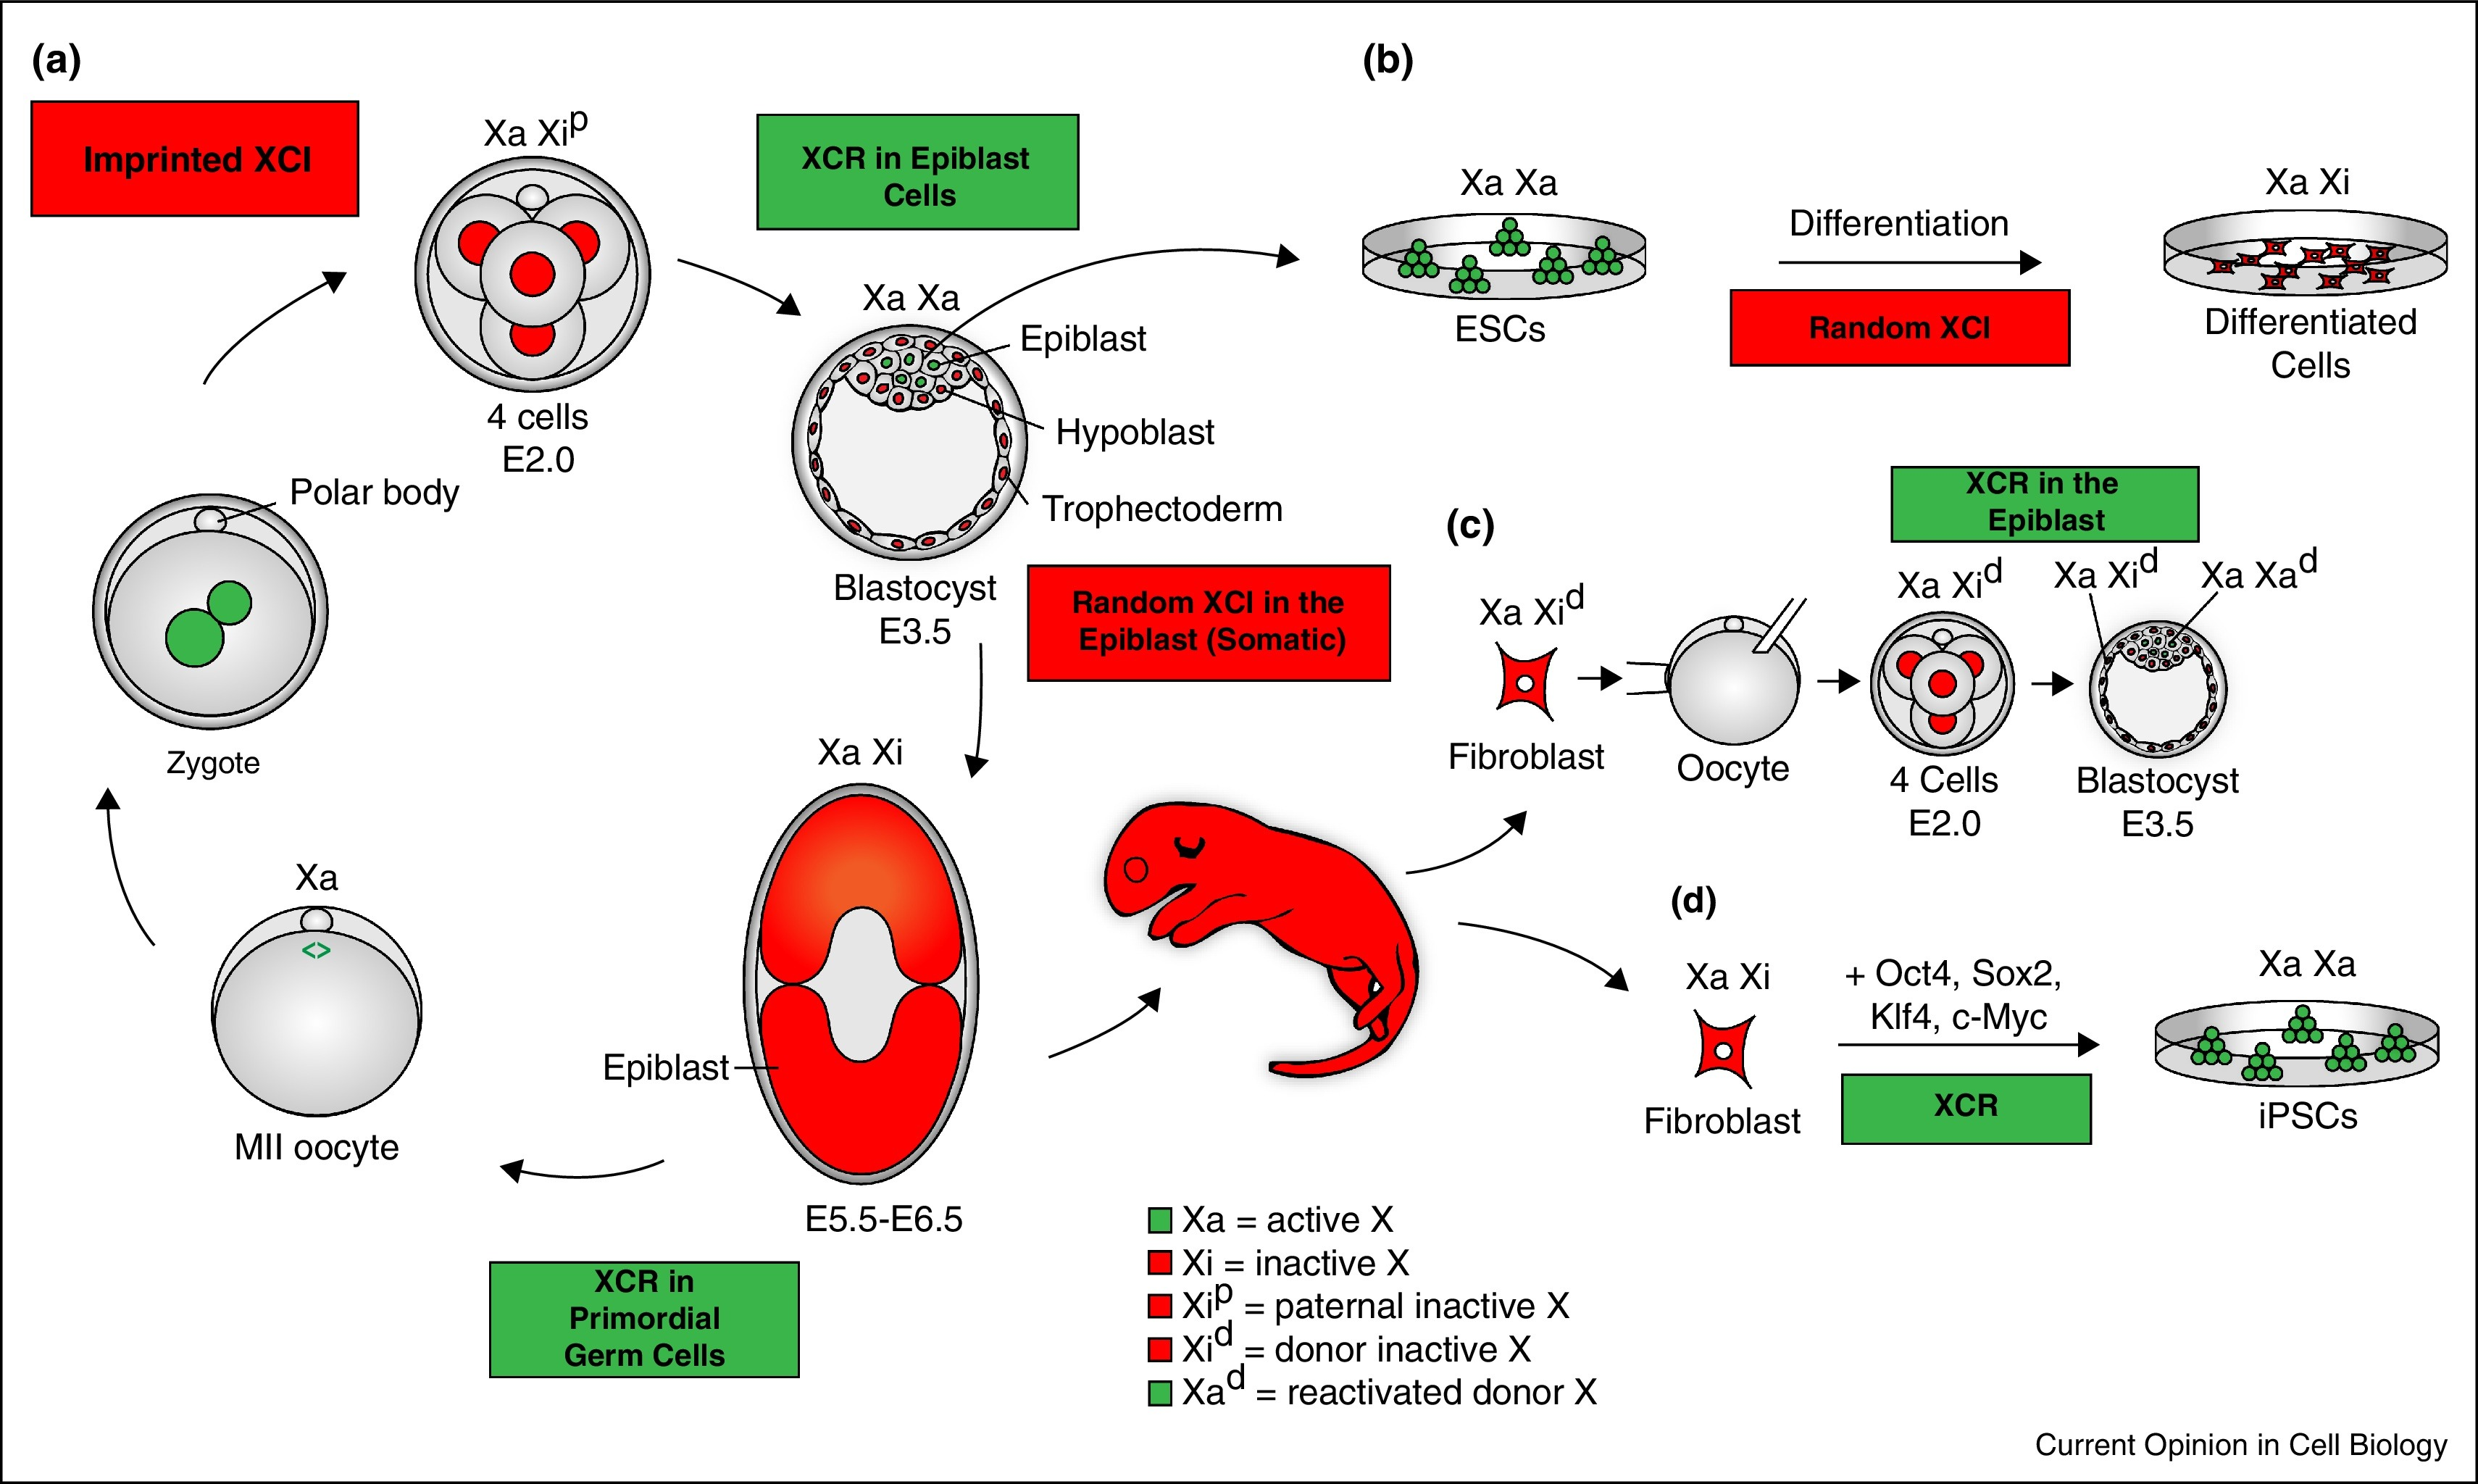
\includegraphics[width=0.75\textwidth]{xcr}
            \caption{X-Chromosome reactivation in mouse embryo and iPSC cells \footcite{XCR} \footnote{Image used from article}}
        \end{figure}
    \end{frame}

    \begin{frame}{Complete reactivation of X-Chromosome}
        \begin{figure}
            \centering
            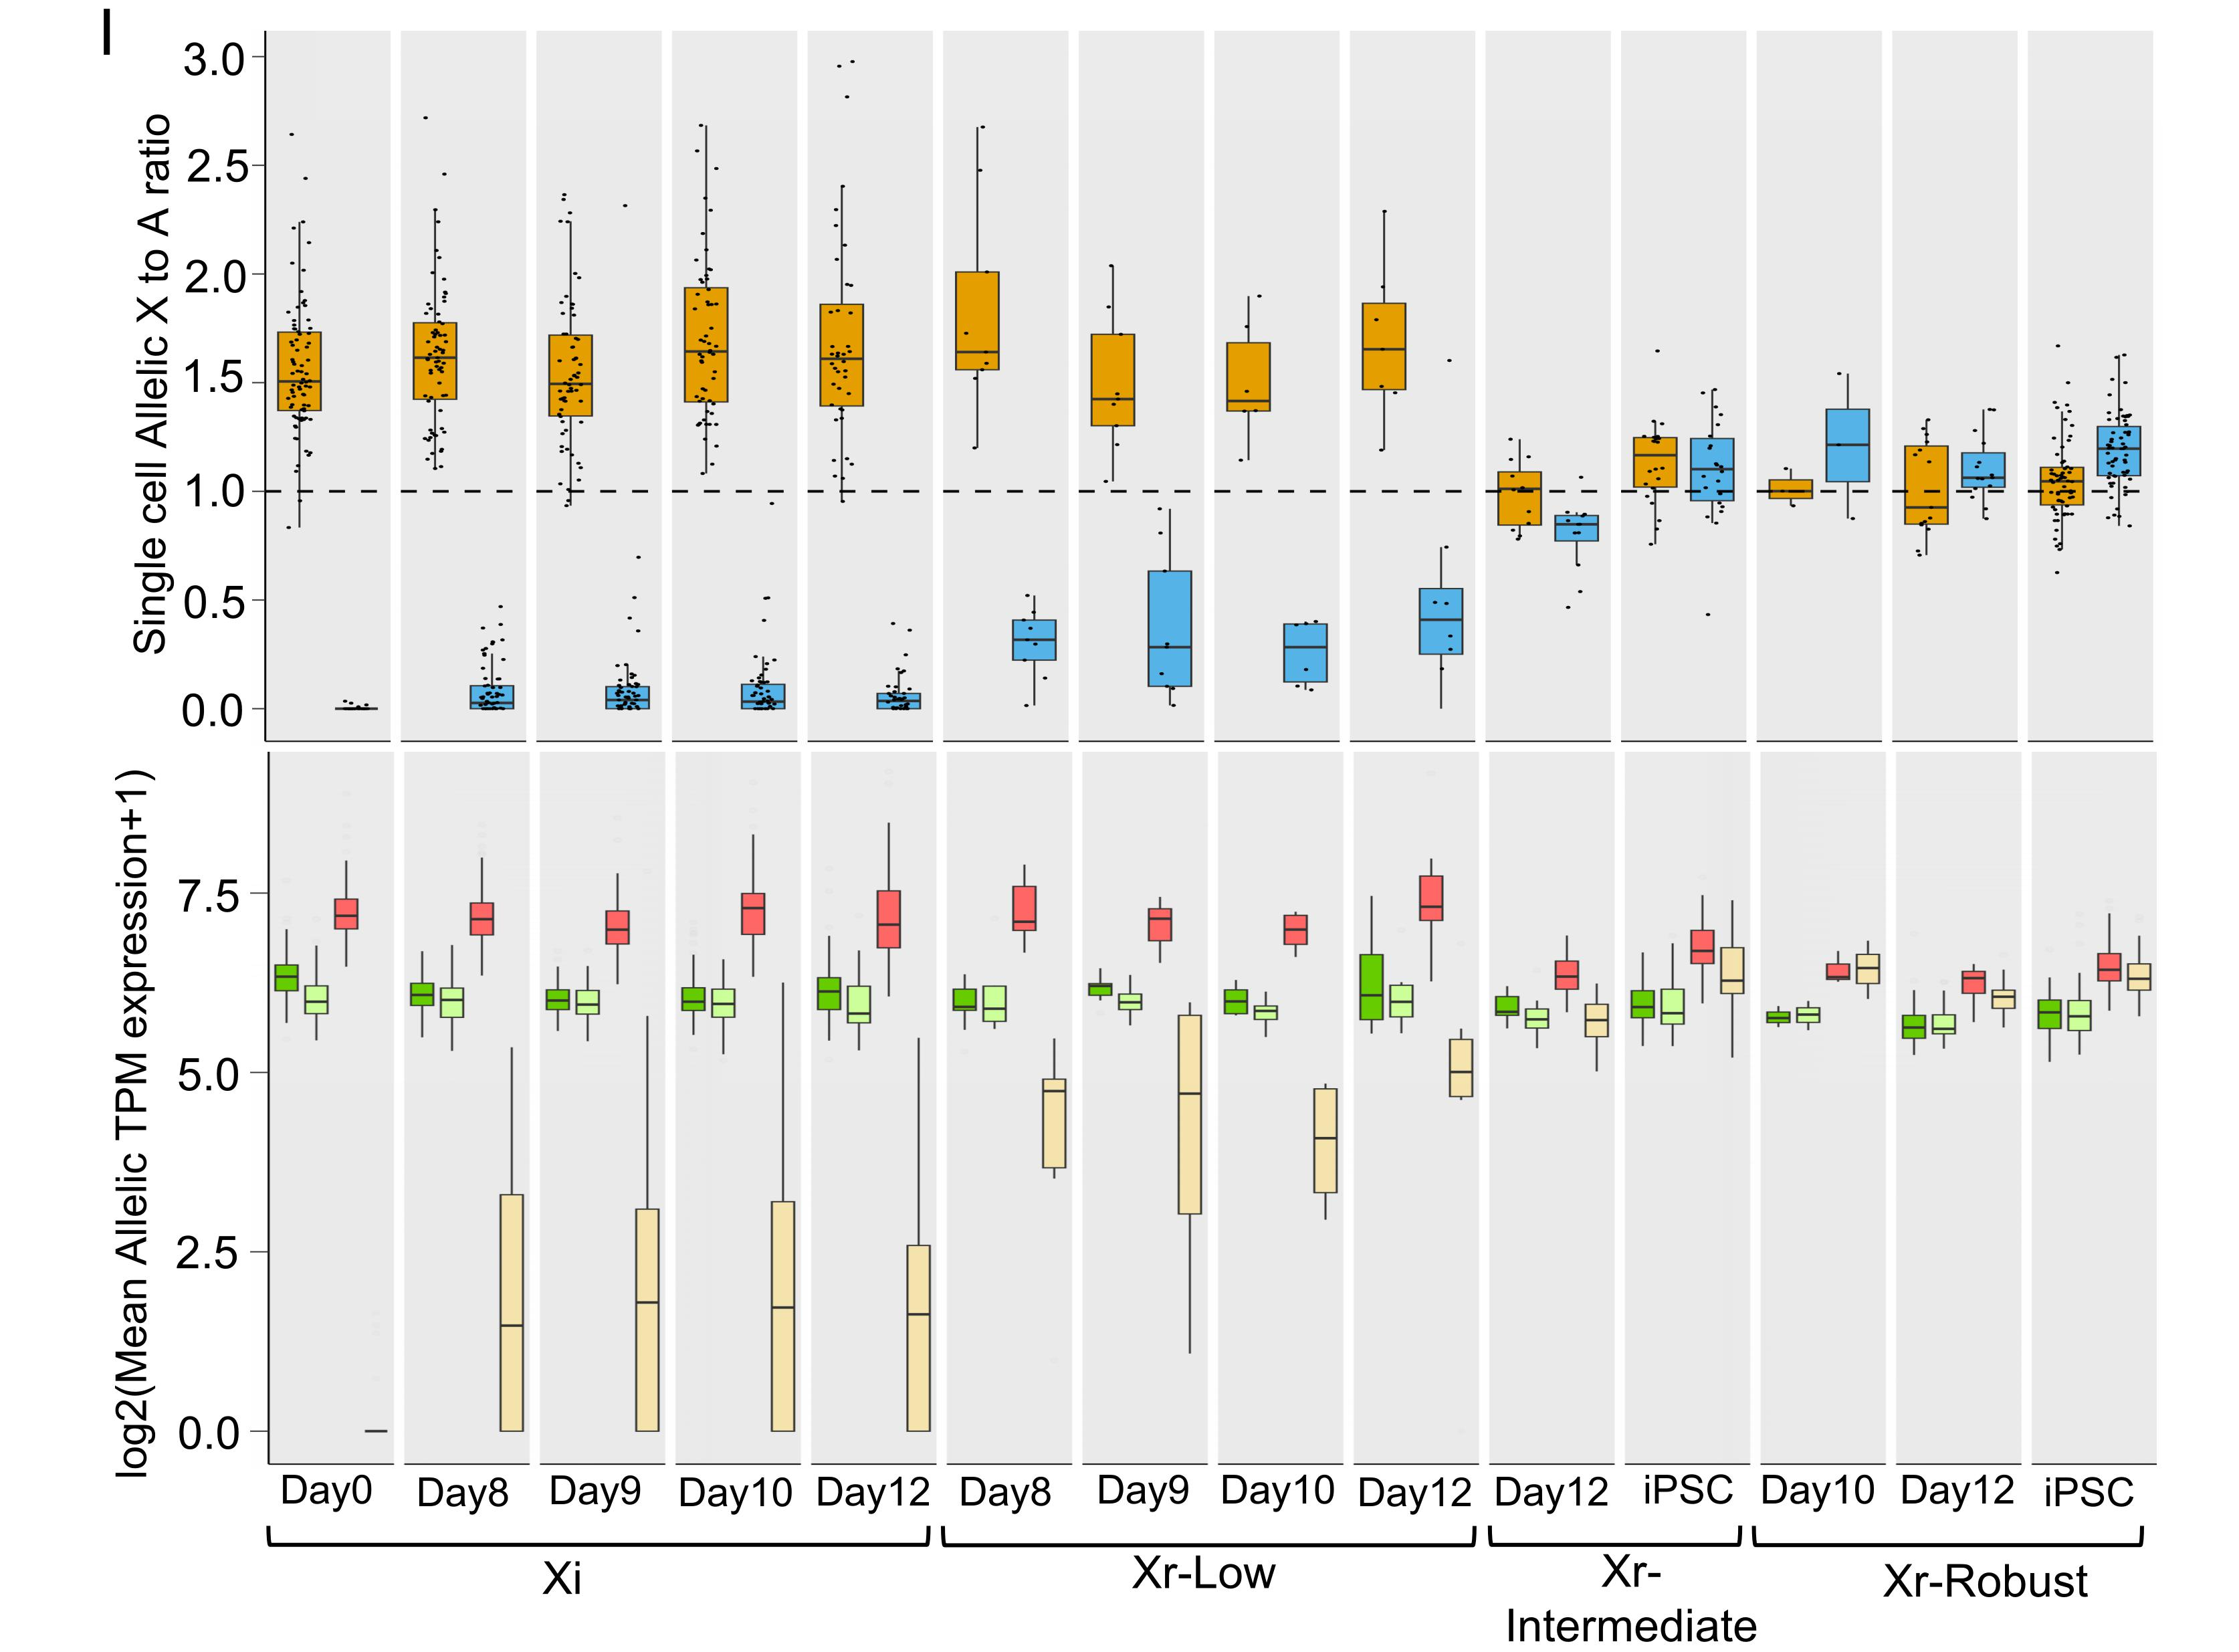
\includegraphics[width=0.6\textwidth]{ipsc}
            \caption{Erasure of X-upregulation on complete reactivation \footnote{Credits: Hemant C. Naik}}
        \end{figure}
    \end{frame}

    \begin{frame}{Partial reactivation of X-Chromosome}
        \begin{figure}
            \centering
            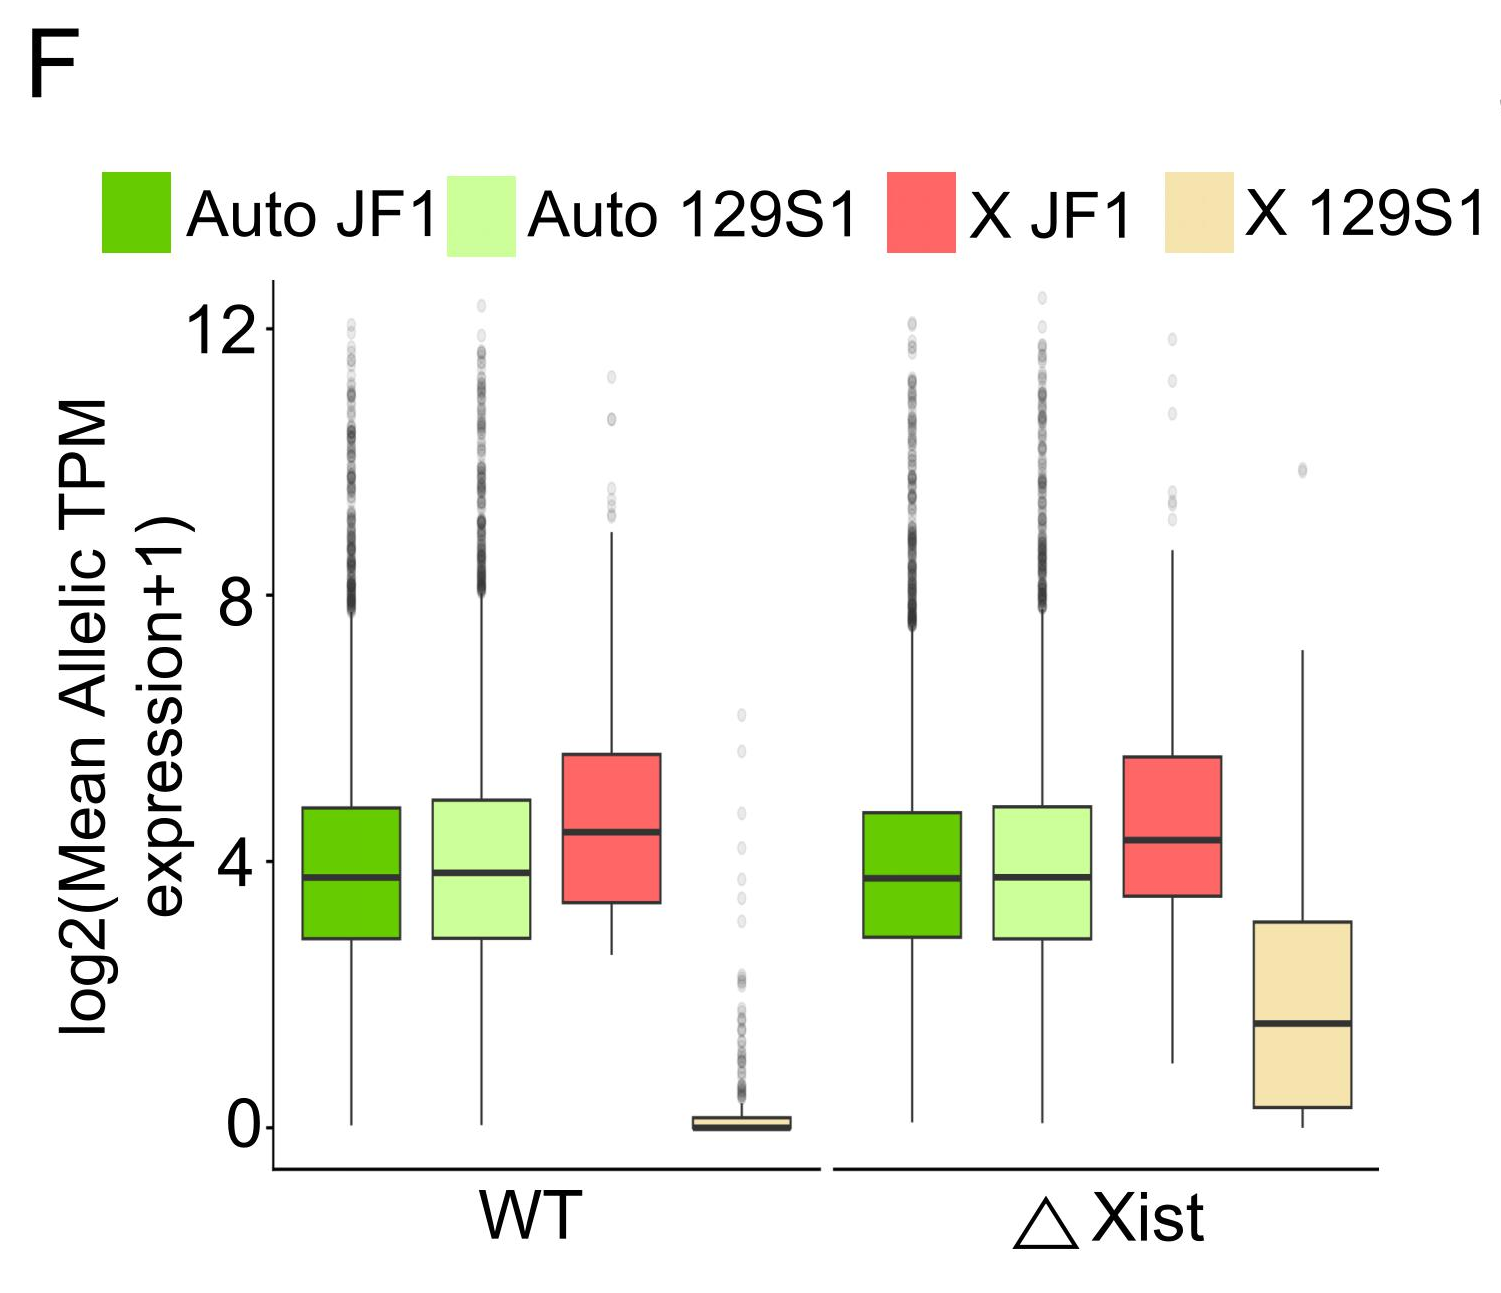
\includegraphics[width=0.5\textwidth]{partial}
            \caption{X-upregulation still present on partial reactivation \footnote{Credits: Hemant C. Naik}}
        \end{figure}
    \end{frame}

    \begin{frame}{Motivation}
        \begin{columns}
            \begin{column}{0.33\textwidth}
                    \begin{figure}
                        \centering
                        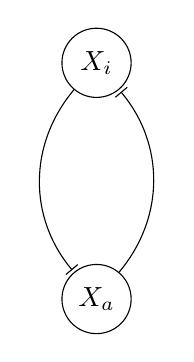
\begin{tikzpicture}[shorten >=1pt,node distance=3cm,on grid,auto]
                            \node[state] (Xi)  {$X_i$};
                            \node[state] (Xa) [below of=Xi] {$X_a$};
                            \path[-|]
                            (Xi) edge [out=230,in=-230]  node {}    (Xa)
                            (Xa) edge [out=50,in=-50]  node {}    (Xi);
                        \end{tikzpicture}
                        \caption{Mutual inhibition?}
                    \end{figure}
                \end{column}
                \begin{column}{0.6\textwidth}
                    \begin{itemize}
                        \item Systems biology approach
                        \item Toggle switch = Bistability during XCI \footcite{XCI-TS}
                        \item Connections influence phenotypes \footcite{topo}
                        \item Simple phenomenological model
                    \end{itemize}
                \end{column}
            \end{columns}
    \end{frame}

    \section{Methods}
    \begin{frame}{Modelling Topologies}
        \begin{columns}
            \begin{column}{0.3\textwidth}
                \begin{figure}
                    \centering
                    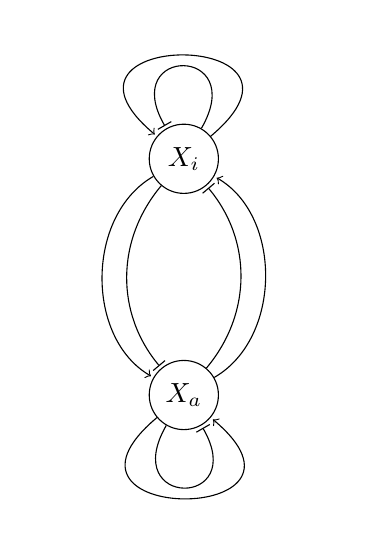
\begin{tikzpicture}[shorten >=1pt,node distance=3cm,on grid,auto]
                        \node[state] (Xi)  {$X_i$};
                        \node[state] (Xa) [below of=Xi] {$X_a$};
                        \path[->]
                            (Xi) edge [out=40,in=140,looseness=8] node {}    (Xi)
                            edge [out=210,in=-210]  node {}    (Xa)
                            (Xa) edge [out=-140,in=-40,looseness=8] node {}    (Xa)
                            edge [out=30,in=-30]  node {}    (Xi);
                        \path[-|]
                        (Xi) edge [out=60,in=120,looseness=7] node {}    (Xi)
                            edge [out=230,in=-230]  node {}    (Xa)
                        (Xa) edge [out=-120,in=-60,looseness=7] node {}    (Xa)
                            edge [out=50,in=-50]  node {}    (Xi);
                    \end{tikzpicture}
                    \caption{Possible topologies}
                \end{figure}
            \end{column}
            \pause
            \begin{column}{0.63\textwidth}
                Differential equations
                \begin{equation}
                    \frac{dX_i}{dt} = \underbrace{a_1\ f(K_1,X_a,n)}_\text{cross} + \underbrace{b_1\ f(K_3,X_i,n)}_\text{self} - \underbrace{c_1 X_i}_\text{decay}
                \end{equation}
                \begin{equation}
                    \frac{dX_a}{dt} = \underbrace{a_2\ f(K_2,X_i,n)}_\text{cross} + \underbrace{b_2\ f(K_4,X_a,n)}_\text{self} - \underbrace{c_2 X_a}_\text{decay}
                \end{equation}
                $$f \in \{ f_a, f_i, f_n\}$$
                \pause
                Activation:
                \begin{equation}
                    f_a(X,K,n) = \frac{{X}^n}{{K}^n+{X}^n}
                \end{equation}
                Inhibition:
                \begin{equation}
                    f_i(X,K,n) = \frac{{K}^n}{{K}^n+{X}^n}
                \end{equation}
                No effect
                \begin{equation}
                    f_n(X,K,n) = 0
                \end{equation}
            \end{column}
        \end{columns}
    \end{frame}

    \begin{frame}{Fitting technique}
        \begin{itemize}
            \item Differential evolution algorithm \footcite{DEalgo}
            \item Sample parameters with Sobol
            \item Solve differential equations with RK45
            \item Calculate sum of square error (residuals)
            \item Generate new parameter set
            \begin{itemize}
                \item Mutation
                \item Crossover
                \item Selection
            \end{itemize}
            \item Repeat till optimal solution
        \end{itemize}
    \end{frame}

    \section{Results}
    \begin{frame}{Preliminary attempts}
        \begin{figure}[h]
            \centering
            \begin{subfigure}[b]{0.49\textwidth}
                \centering
                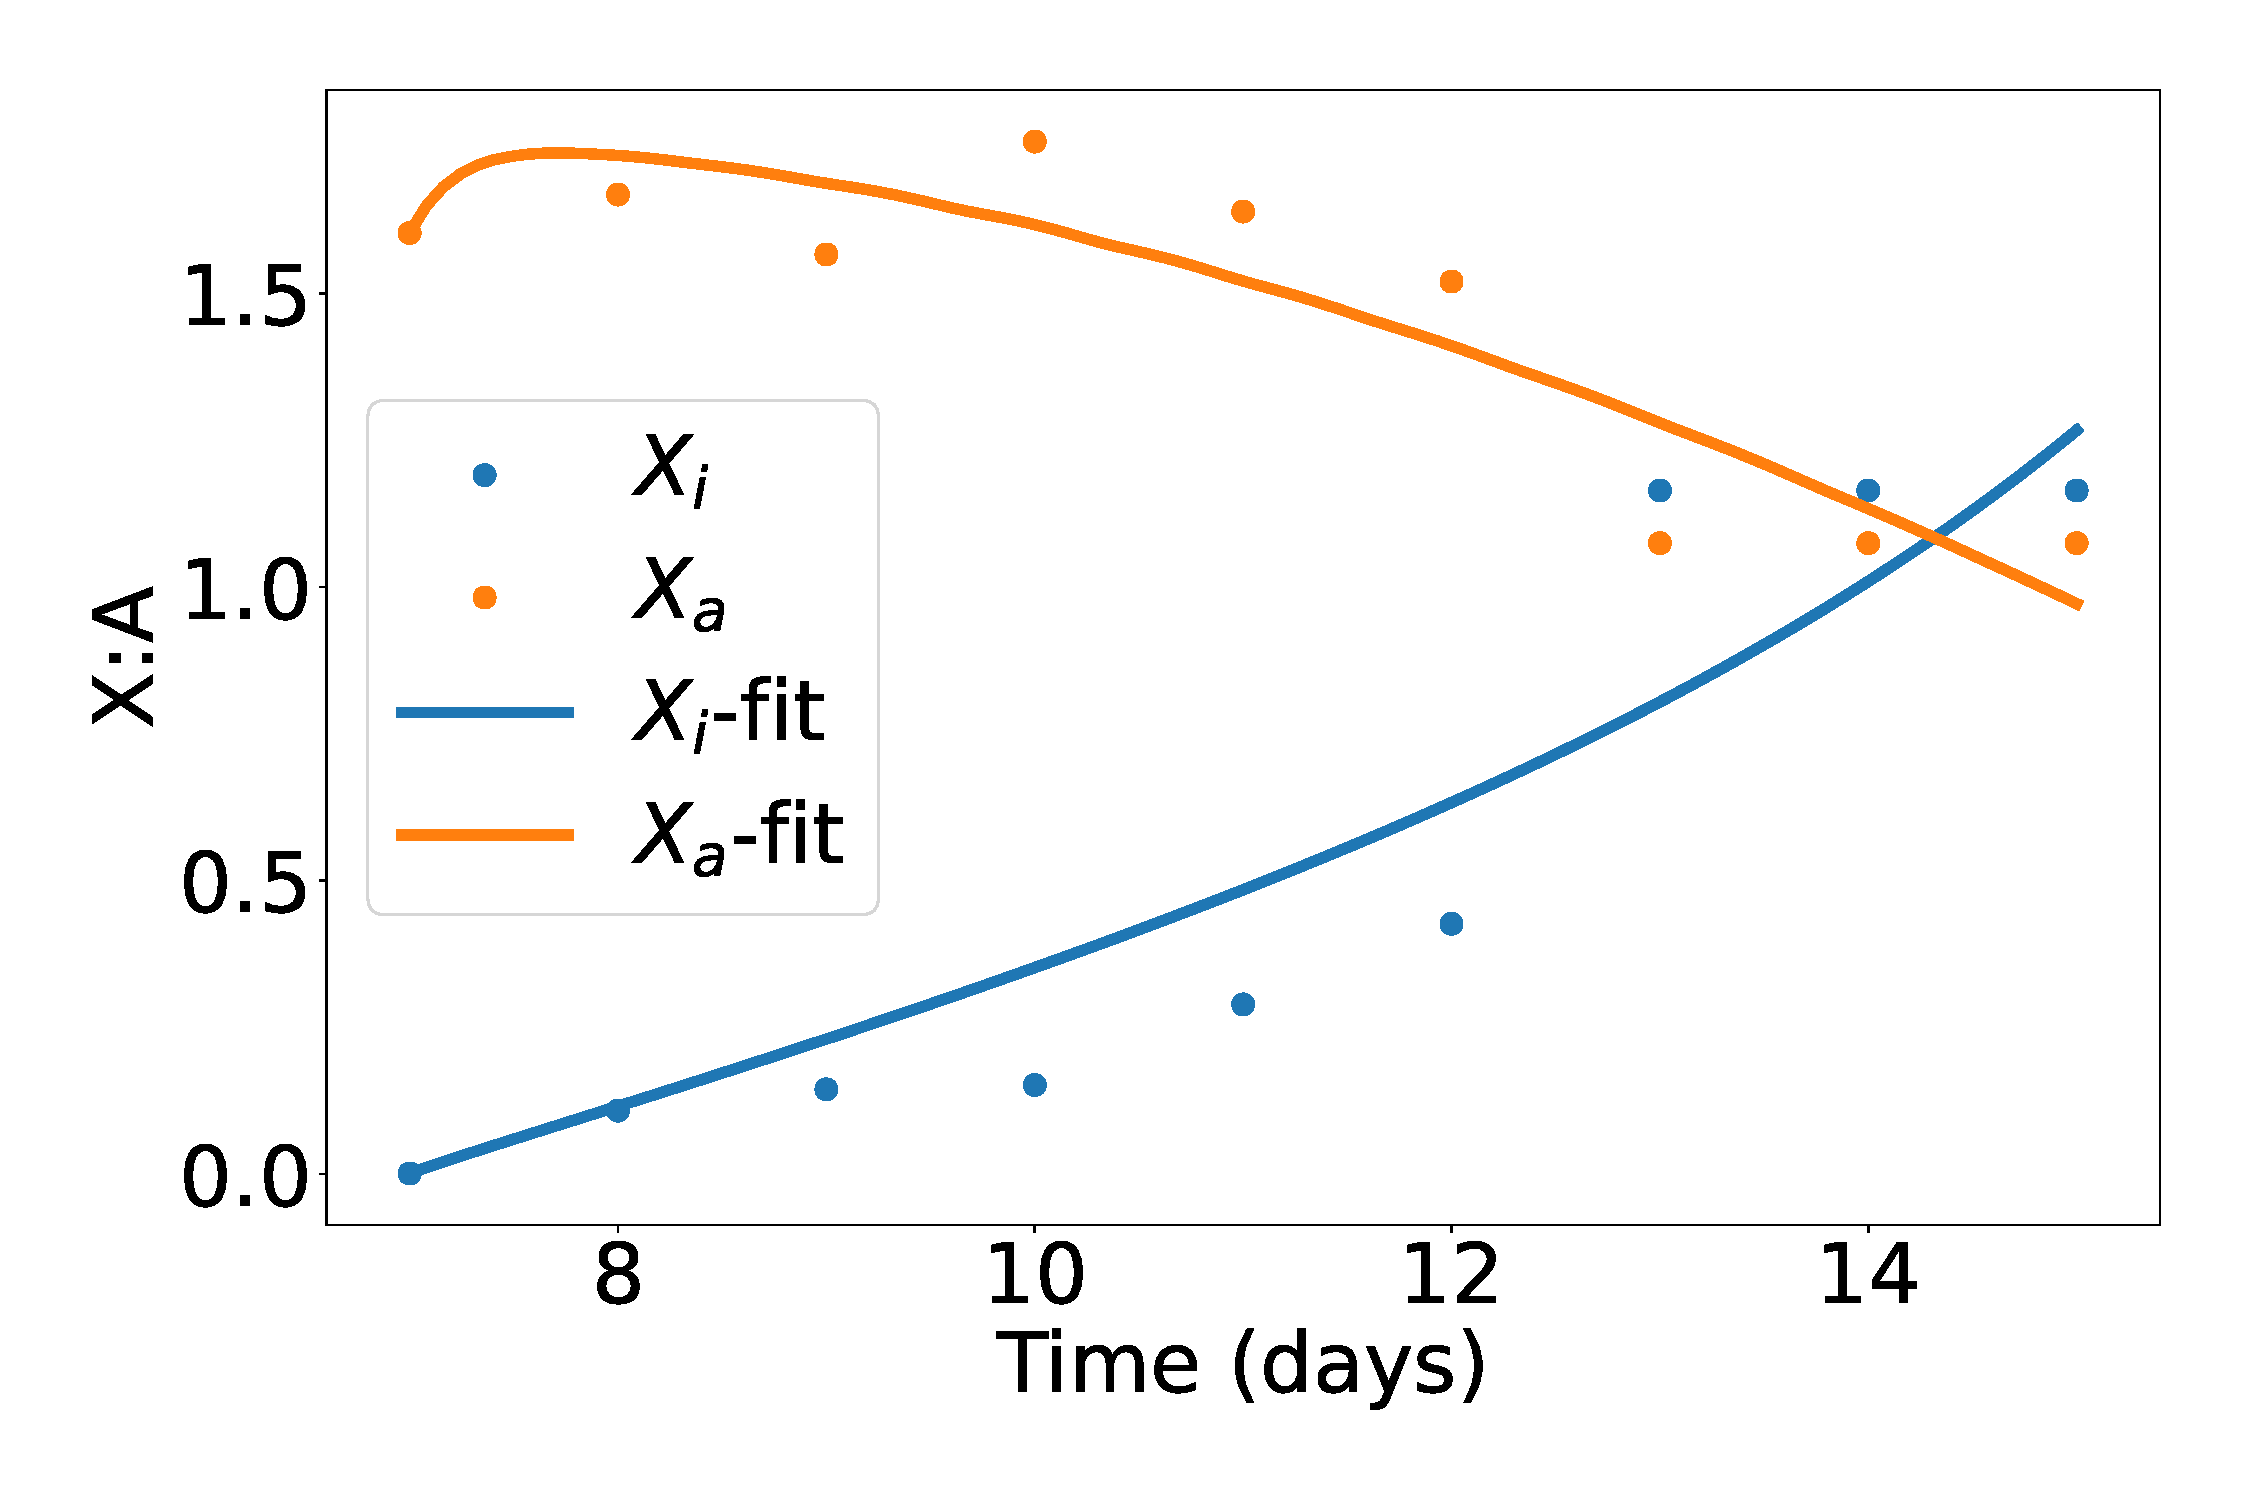
\includegraphics[width=\textwidth]{IINN-iPSC_timeshifted-timeseries}
                \caption{Cross-inhibition}
            \end{subfigure}
            \caption{Fits on Full reactivation: iPSC induction data}
        \end{figure}
    \end{frame}

    \begin{frame}{Preliminary attempts}  
        \begin{figure}[h]\ContinuedFloat
            \begin{subfigure}[b]{0.49\textwidth}
                \centering
                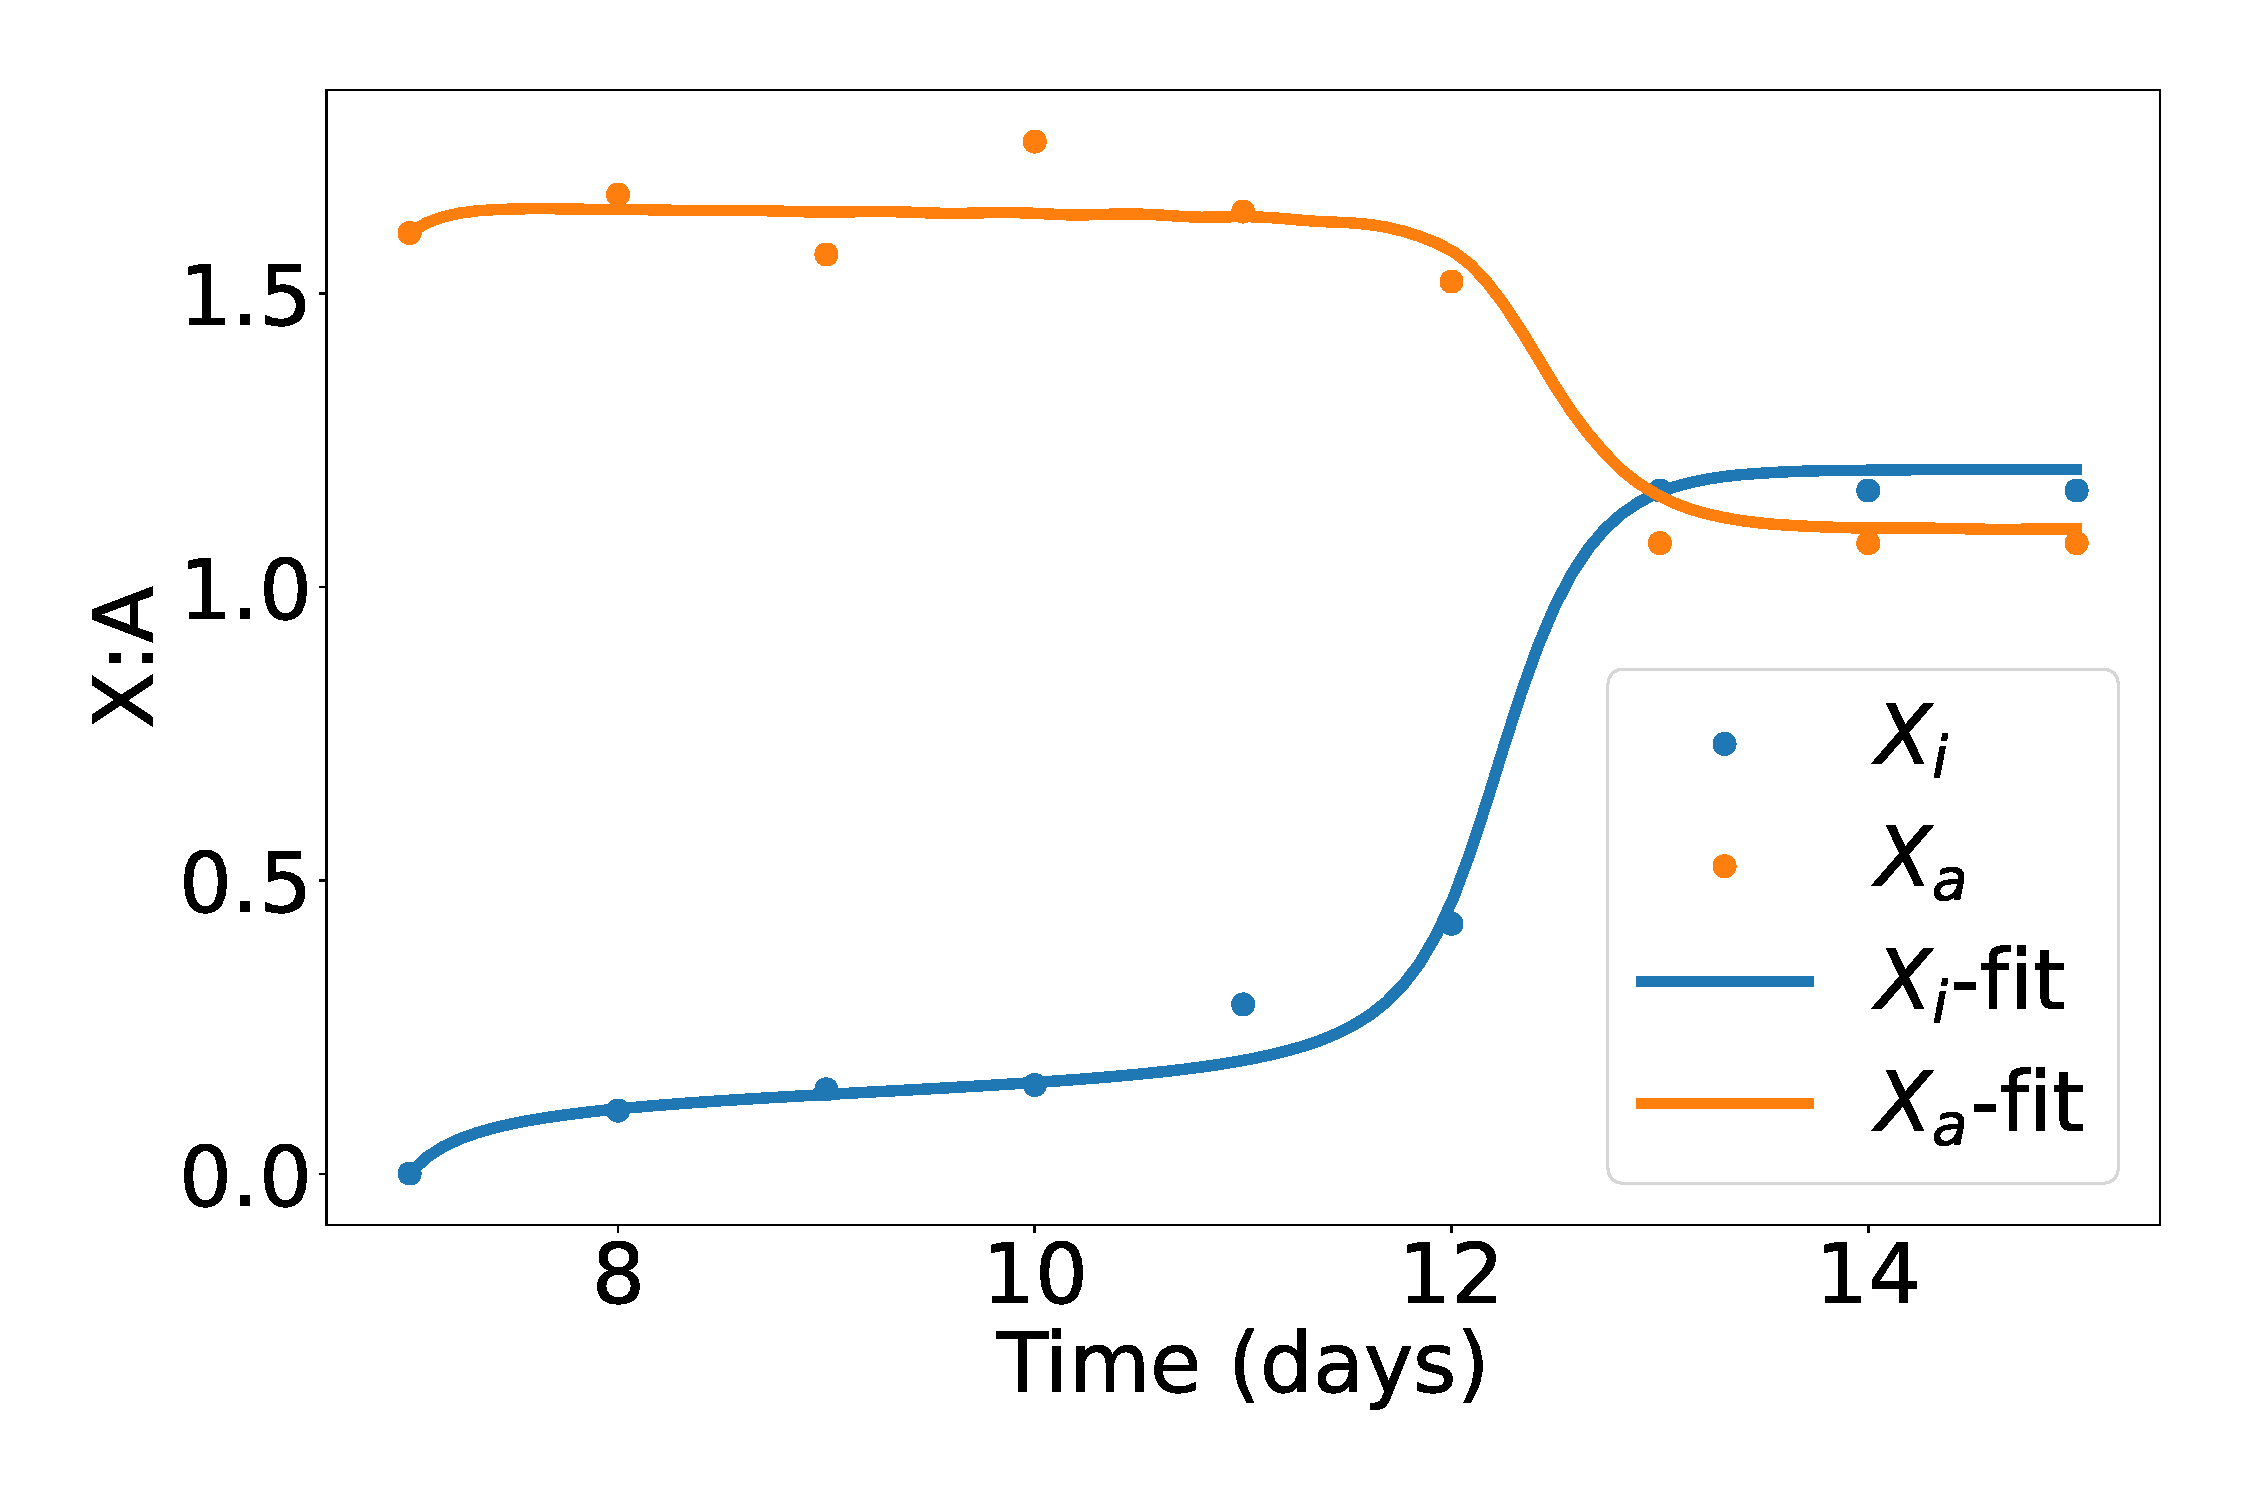
\includegraphics[width=\textwidth]{IIAA-iPSC_timeshifted-timeseries}
                \caption{Cross-inhibition with self-activation}
            \end{subfigure}
            \begin{subfigure}[b]{0.49\textwidth}
                \centering
                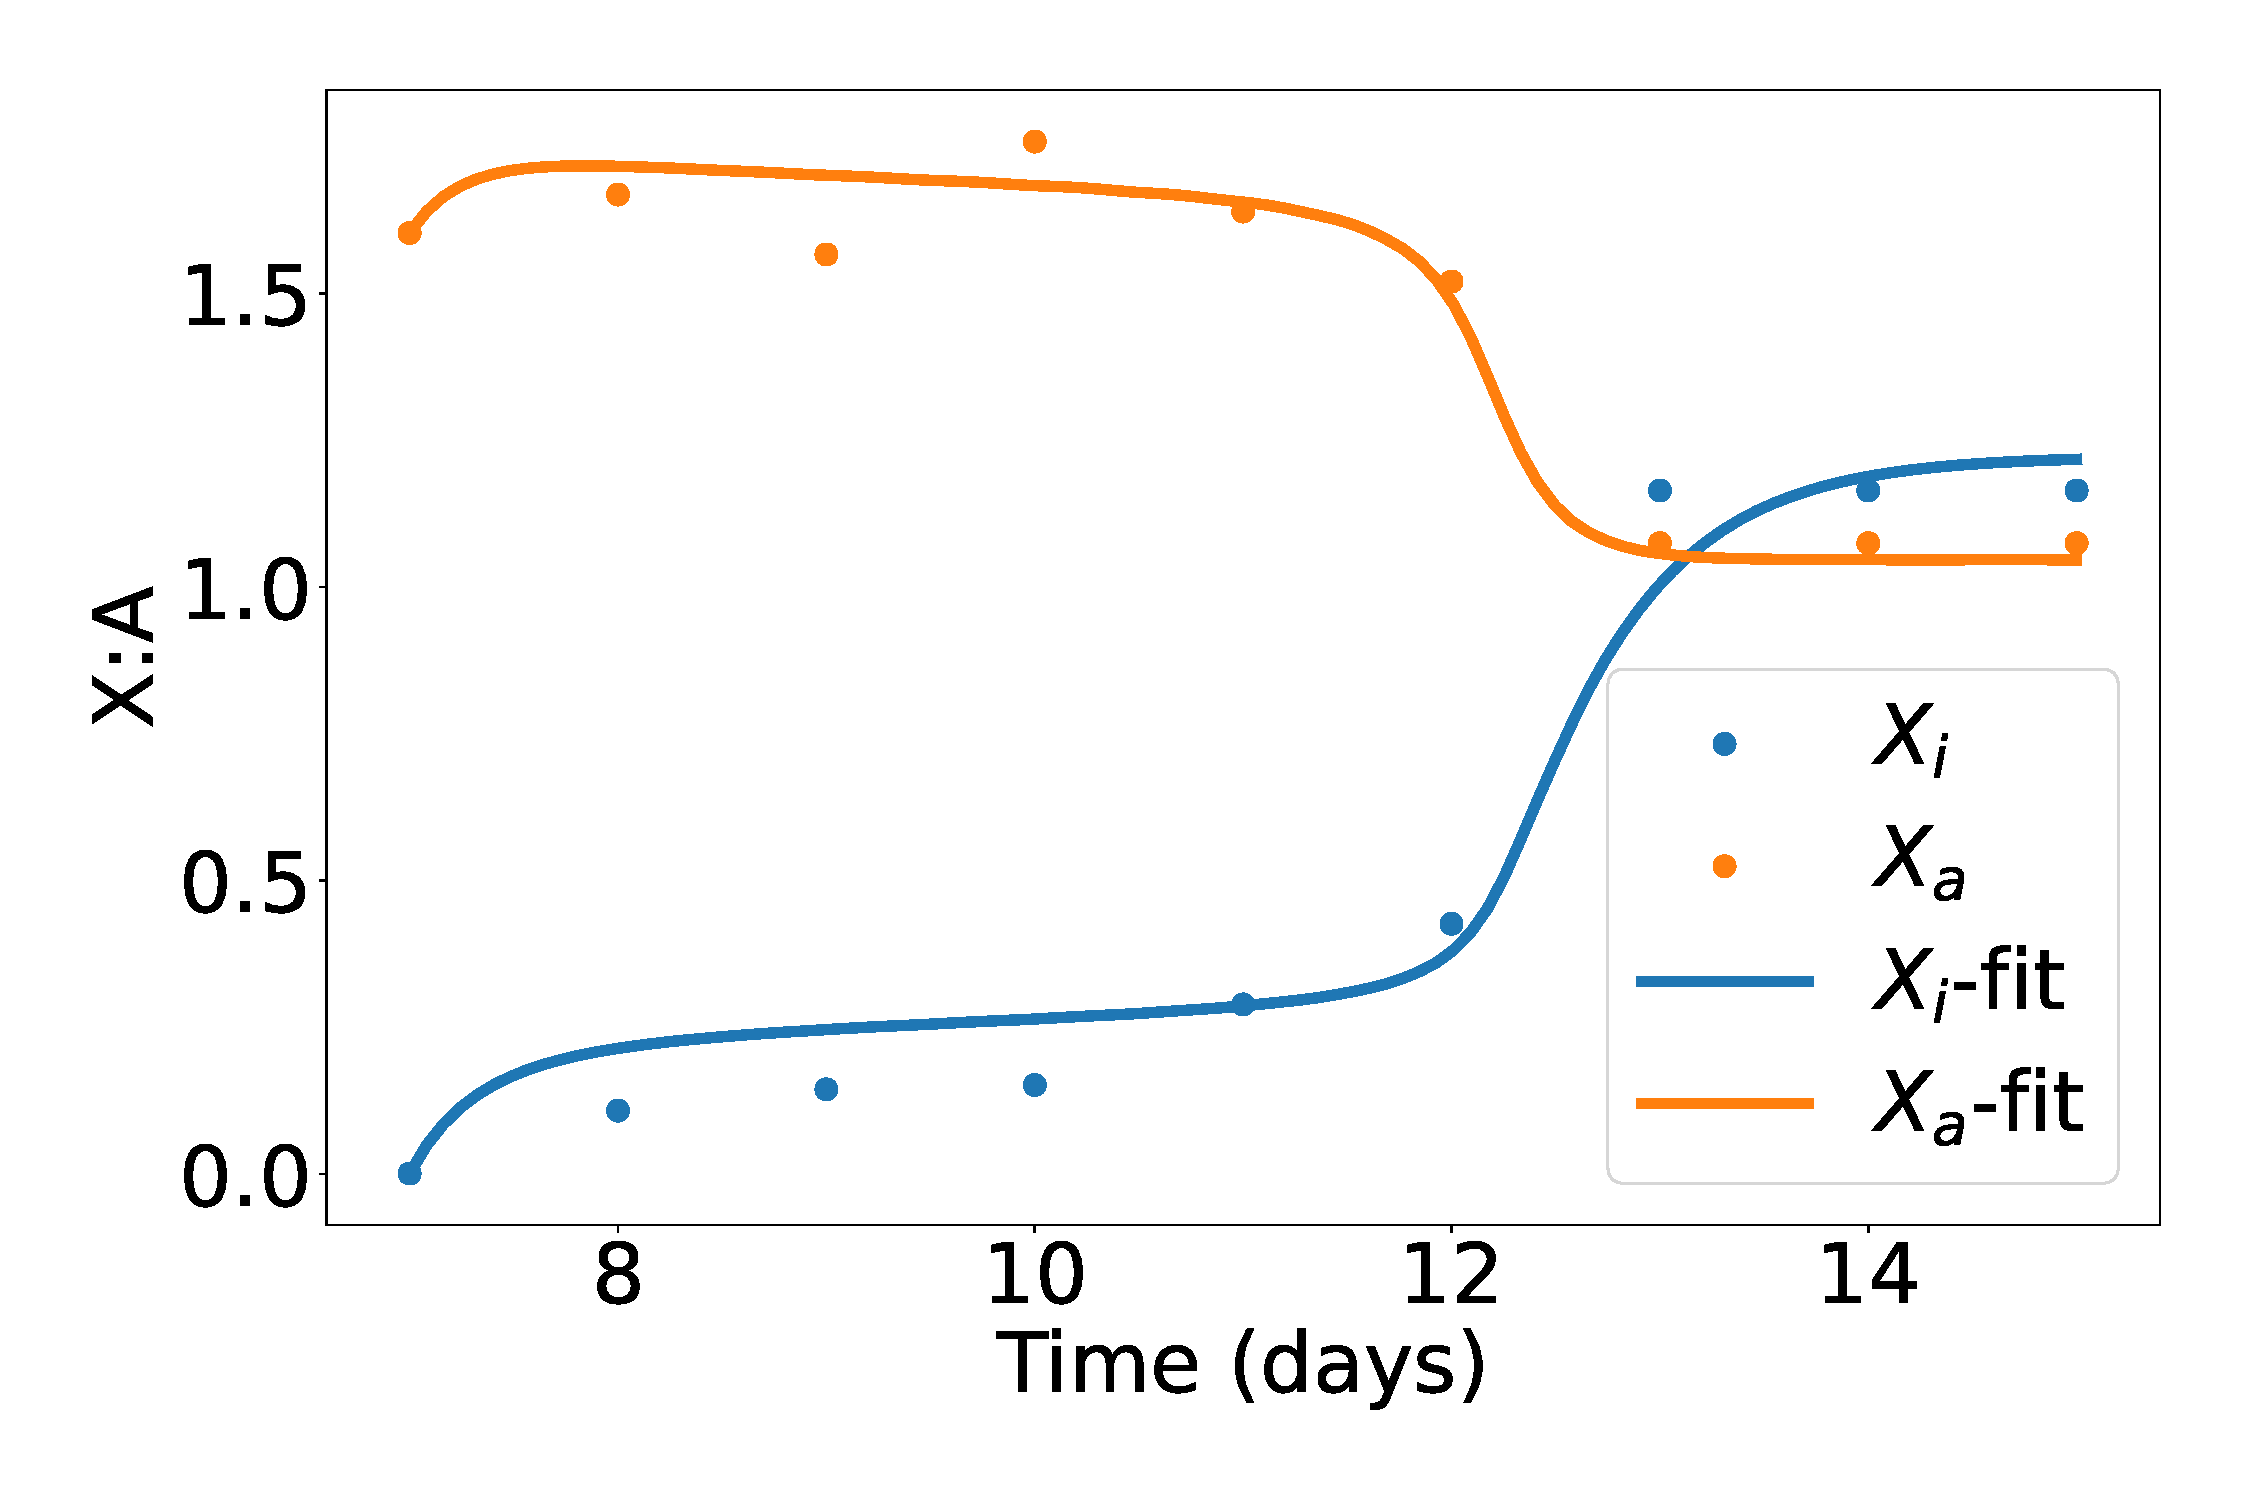
\includegraphics[width=\textwidth]{IIII-iPSC_timeshifted-timeseries}
                \caption{Cross-inhibition with self-inhibition}
            \end{subfigure}
            \caption{Fits on Full reactivation: iPSC induction data}
        \end{figure}
    \end{frame}

    \begin{frame}{Testing self connections w/ fixed cross-inhibition}
        \begin{columns}
            \begin{column}{0.23\textwidth}
                \begin{figure}[h]
                    \centering
                    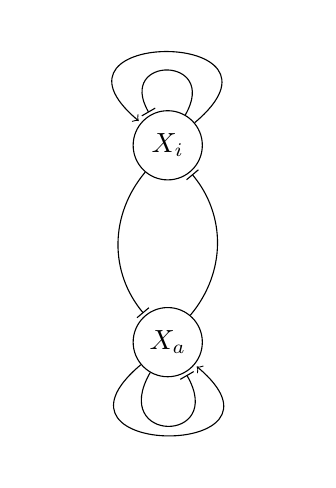
\begin{tikzpicture}[shorten >=1pt,node distance=2.5cm,on grid,auto]
                        \node[state] (Xi)  {$X_i$};
                        \node[state] (Xa) [below of=Xi] {$X_a$};
                        \path[->]
                            (Xi) edge [out=40,in=140,looseness=7] node {}    (Xi)
                            (Xa) edge [out=-140,in=-40,looseness=7] node {}    (Xa);
                        \path[-|]
                        (Xi) edge [out=60,in=120,looseness=5] node {}    (Xi)
                            edge [out=230,in=-230]  node {}    (Xa)
                        (Xa) edge [out=-120,in=-60,looseness=6] node {}    (Xa)
                            edge [out=50,in=-50]  node {}    (Xi);
                    \end{tikzpicture}
                    \caption{Self connections}
                \end{figure}
            \end{column}
            \pause
            \begin{column}{0.75\textwidth}
                \begin{figure}[h]
                        \centering
                        \begin{subfigure}[b]{0.49\textwidth}
                            \centering
                            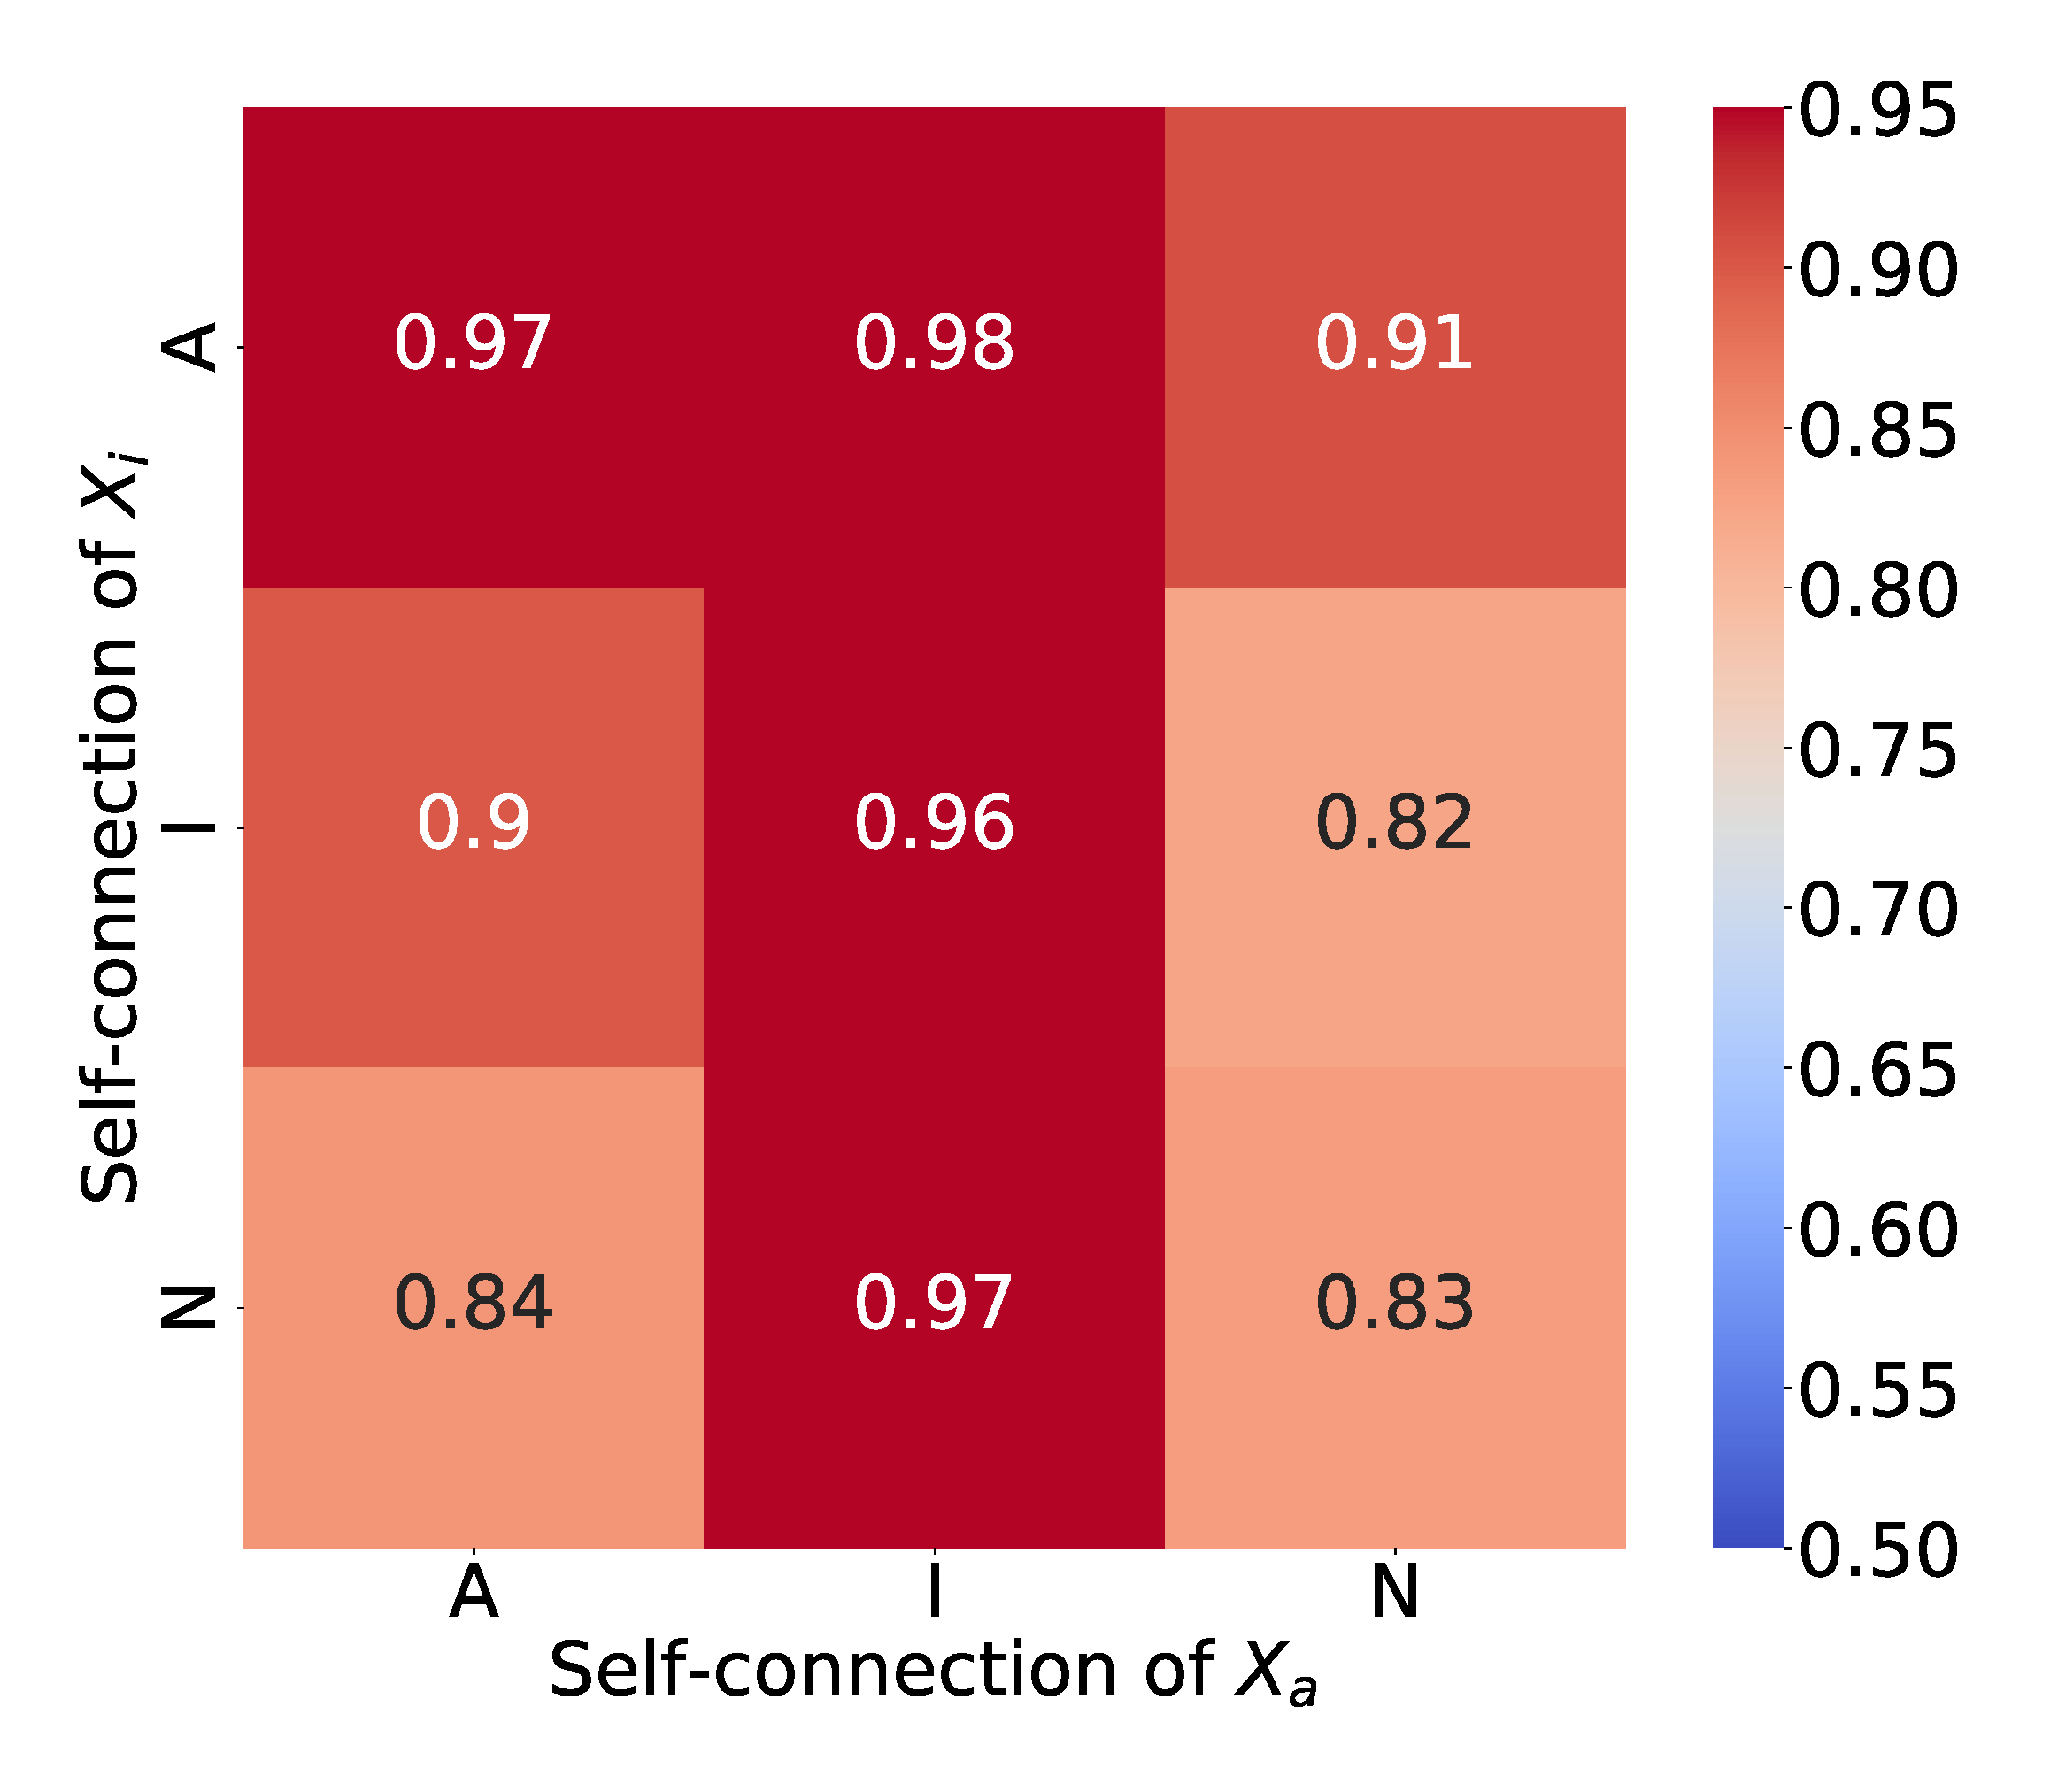
\includegraphics[width=\textwidth]{vary_self-iPSC_timeshifted-rsq-hmap}
                            \caption{Full reactivation}
                        \end{subfigure}
                        \pause
                        \begin{subfigure}[b]{0.49\textwidth}
                            \centering
                            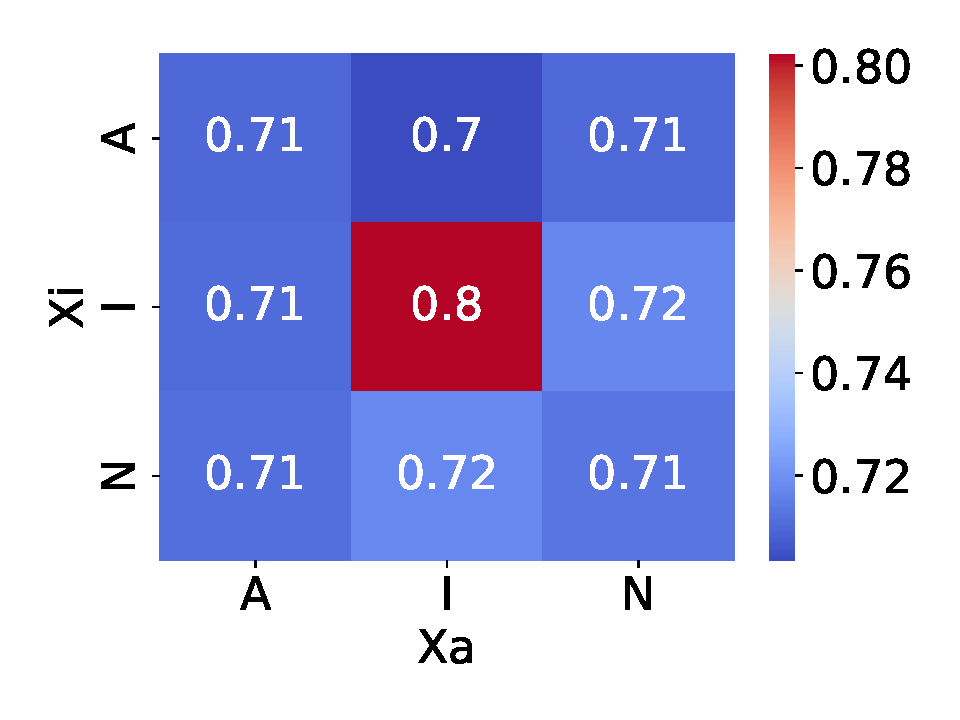
\includegraphics[width=\textwidth]{vary_self-Partial_timeshifted-rsq-hmap}
                            \caption{Partial reactivation}
                        \end{subfigure}
                    \pause[2]\caption{Heatmaps of $R^2$ values}
                \end{figure}
            \end{column}
        \end{columns}
    \end{frame}

    \begin{frame}{Plots of timeseries with fits}
        \begin{figure}[h]
            \centering
            \begin{subfigure}[b]{0.49\textwidth}
                \centering
                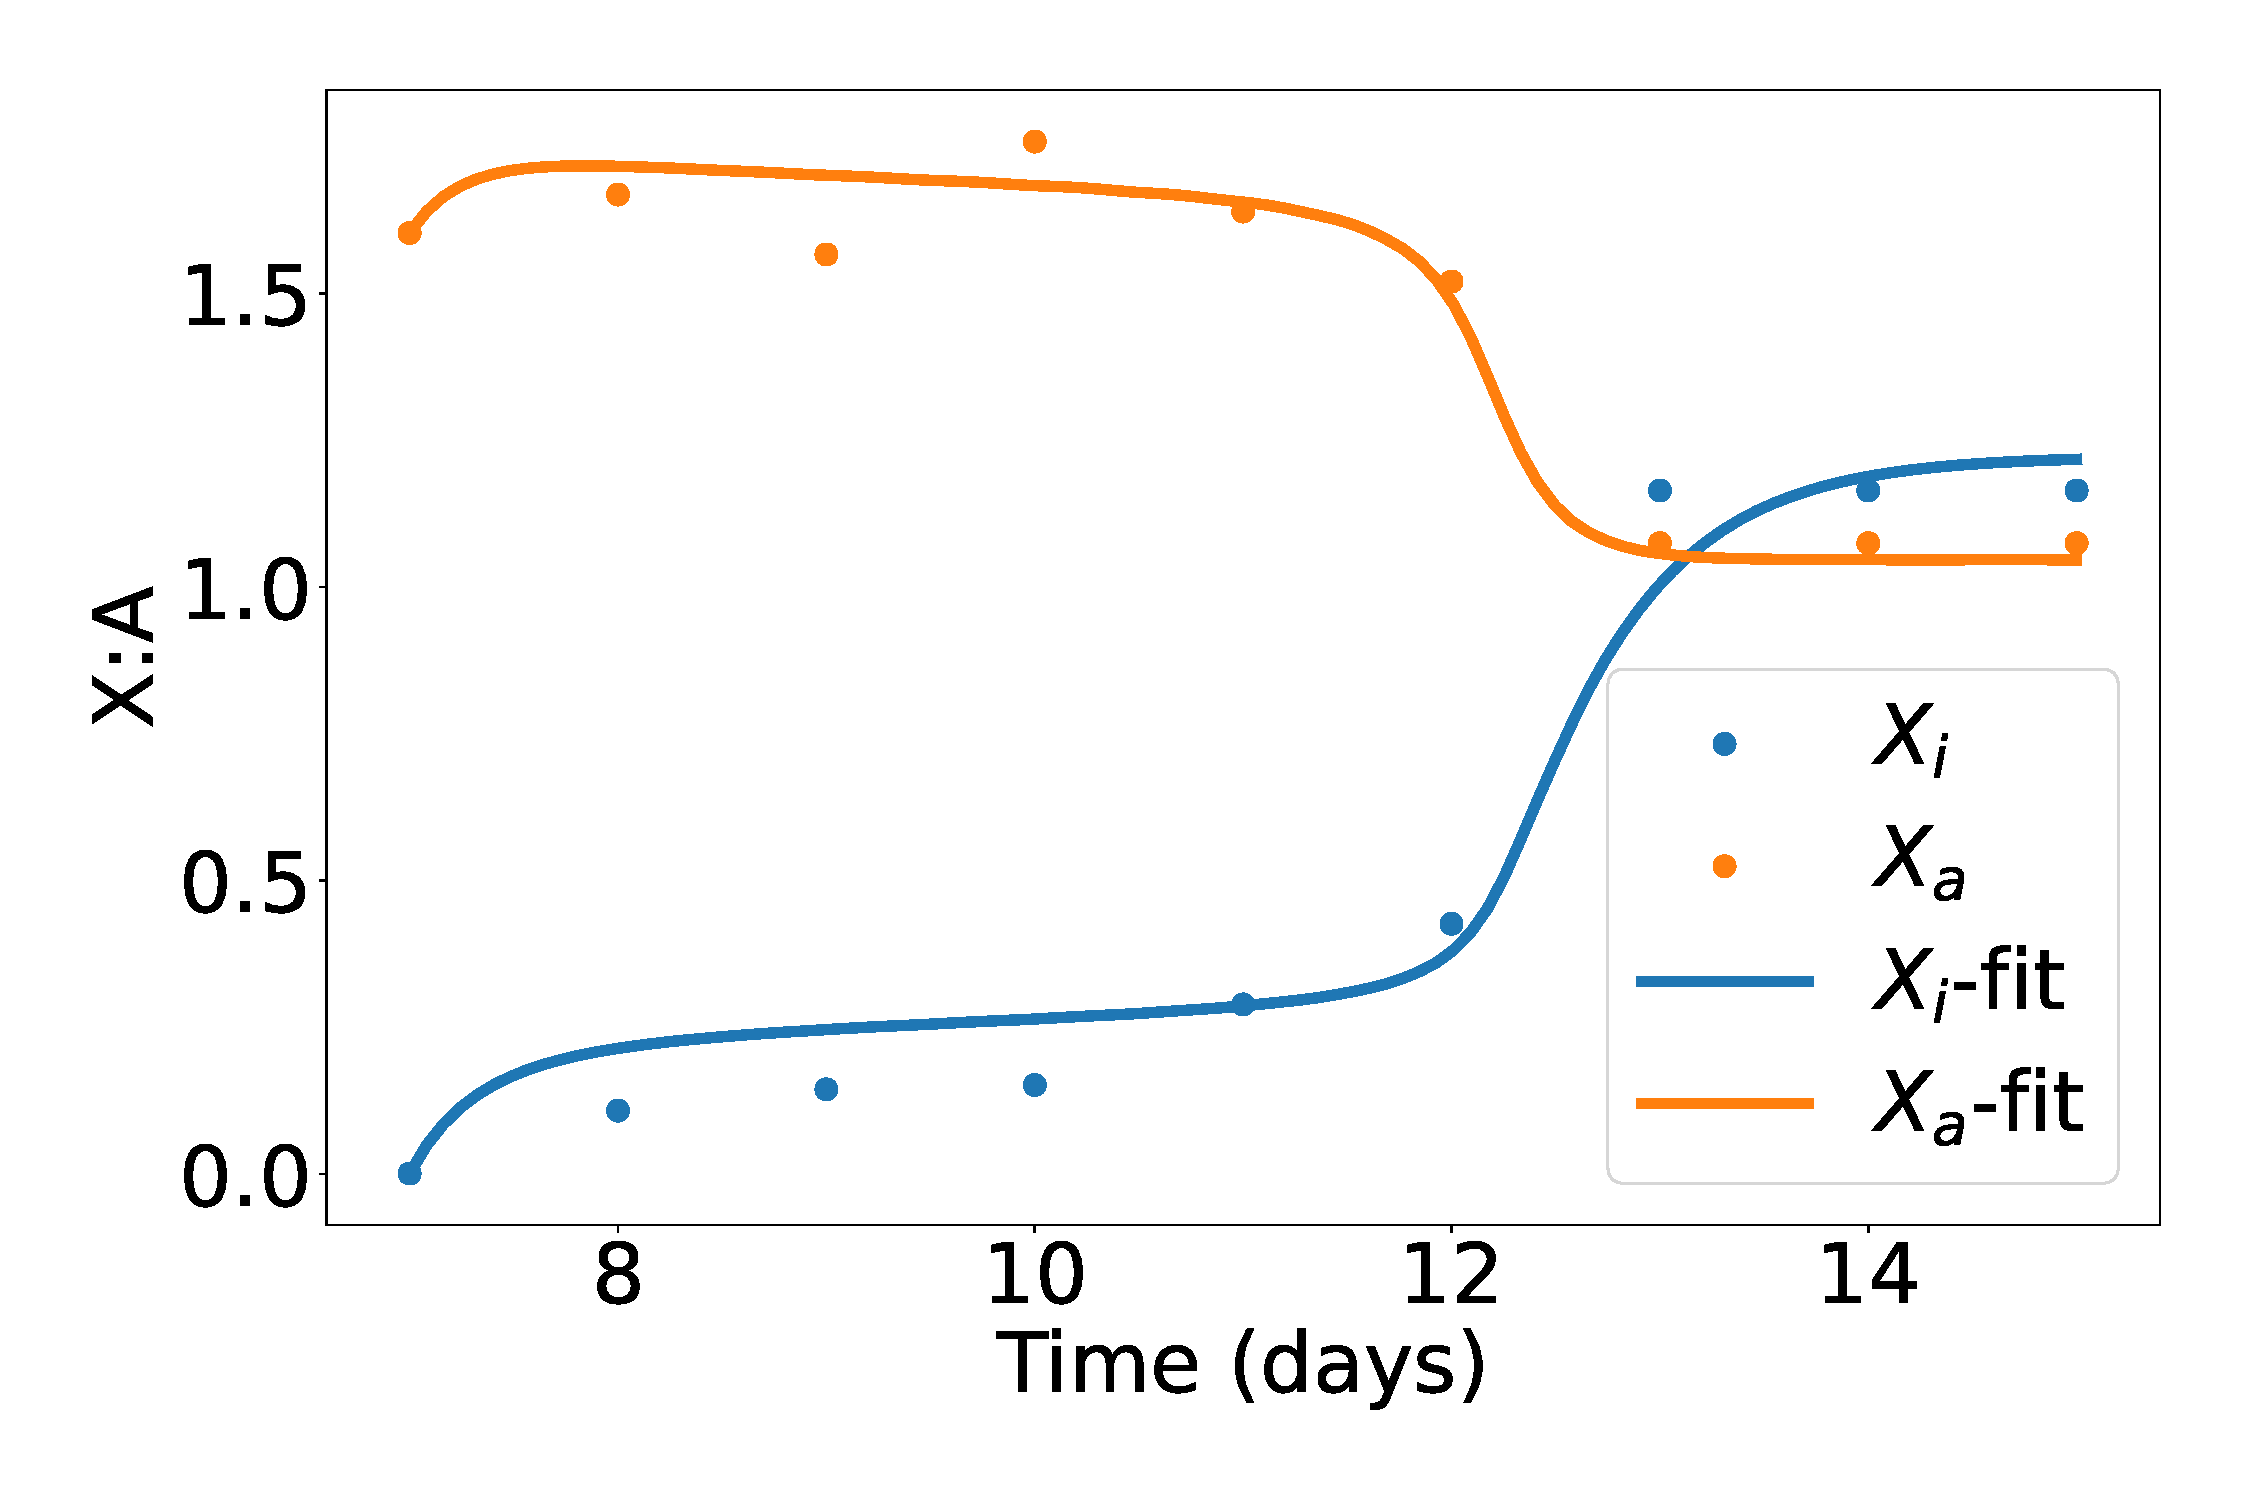
\includegraphics[width=\textwidth]{IIII-iPSC_timeshifted-timeseries}
                \caption{Complete reactivation}
            \end{subfigure}
            \begin{subfigure}[b]{0.49\textwidth}
                \centering
                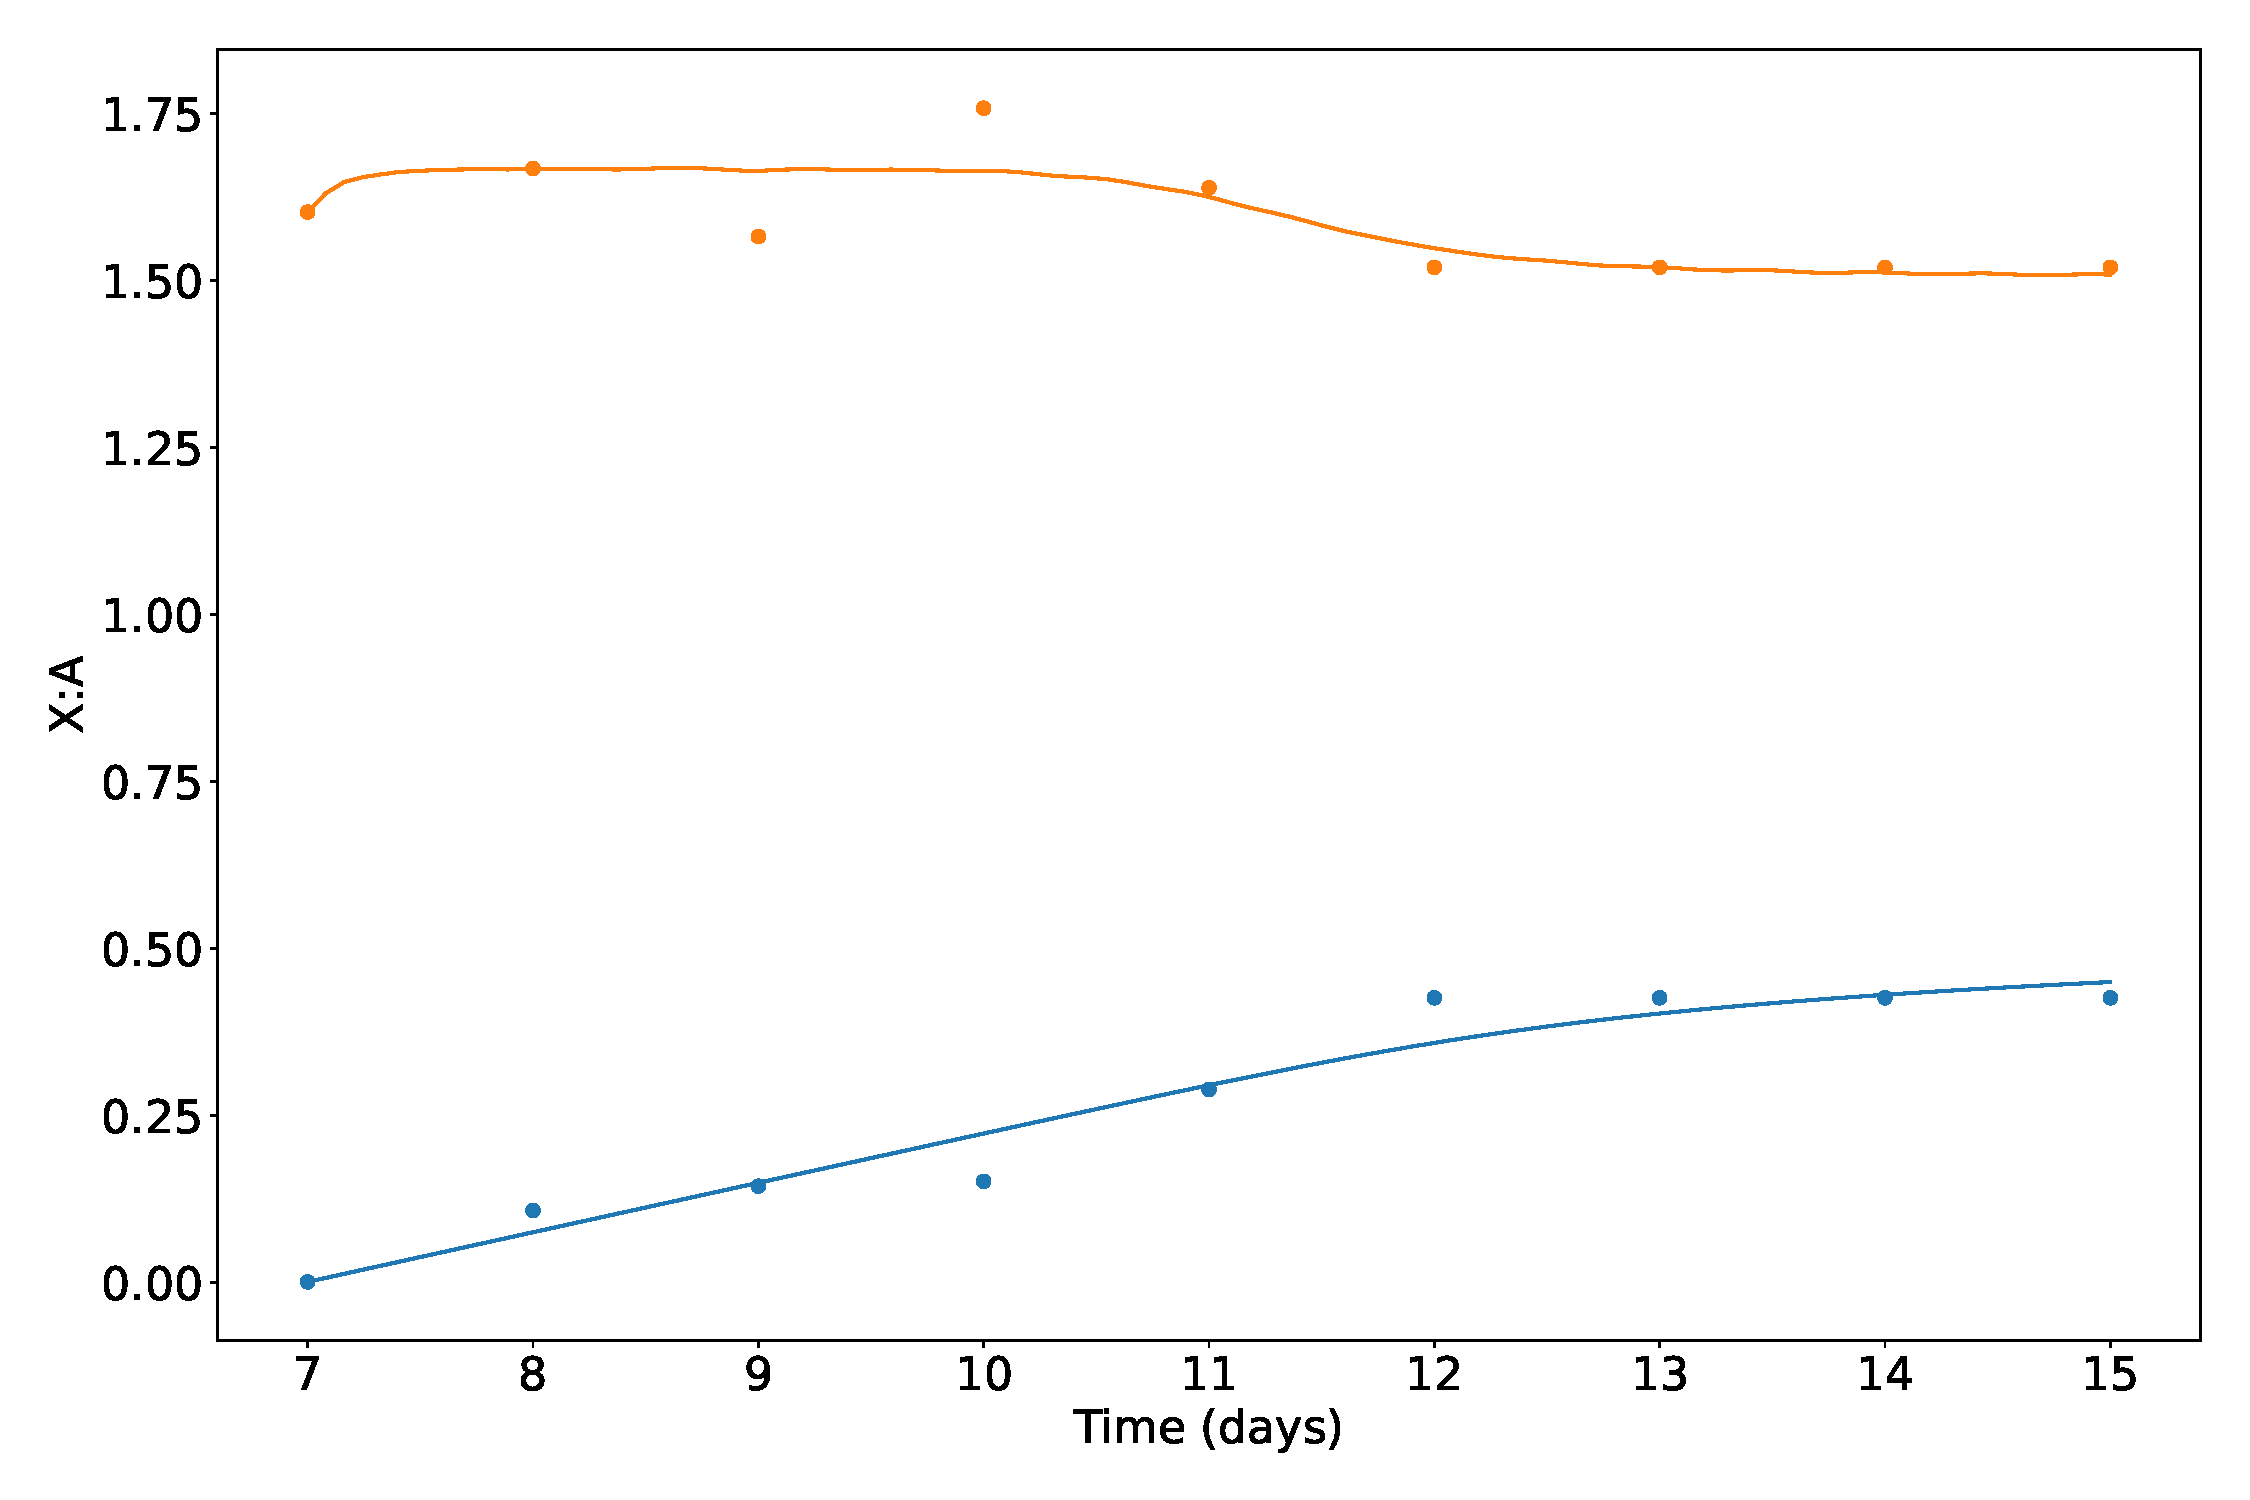
\includegraphics[width=\textwidth]{IIII-Partial_timeshifted-timeseries}
                \caption{Partial reactivation}
            \end{subfigure}
            \caption{Timeseries with fits of cross-inhibition with self-inhibition}
        \end{figure}
    \end{frame}

    \begin{frame}{Testing cross connections w/ fixed self-inhibition}
        \begin{columns}
            \begin{column}{0.3\textwidth}
                \begin{figure}
                    \centering
                    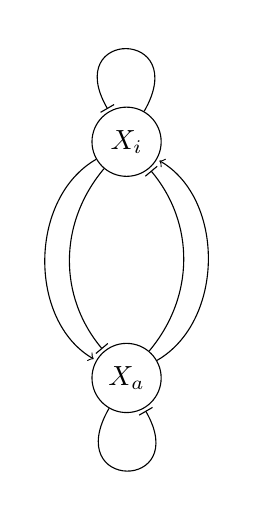
\begin{tikzpicture}[shorten >=1pt,node distance=3cm,on grid,auto]
                        \node[state] (Xi)  {$X_i$};
                        \node[state] (Xa) [below of=Xi] {$X_a$};
                        \path[->]
                            (Xi) edge [out=210,in=-210]  node {}    (Xa)
                            (Xa) edge [out=30,in=-30]  node {}    (Xi);
                        \path[-|]
                        (Xi) edge [out=60,in=120,looseness=7] node {}    (Xi)
                            edge [out=230,in=-230]  node {}    (Xa)
                        (Xa) edge [out=-120,in=-60,looseness=7] node {}    (Xa)
                            edge [out=50,in=-50]  node {}    (Xi);
                    \end{tikzpicture}
                    \caption{Cross connections}
                \end{figure}
            \end{column}
            \pause
            \begin{column}{0.62\textwidth}
                \begin{figure}[h]
                        \centering
                        \begin{subfigure}[b]{0.49\textwidth}
                            \centering
                            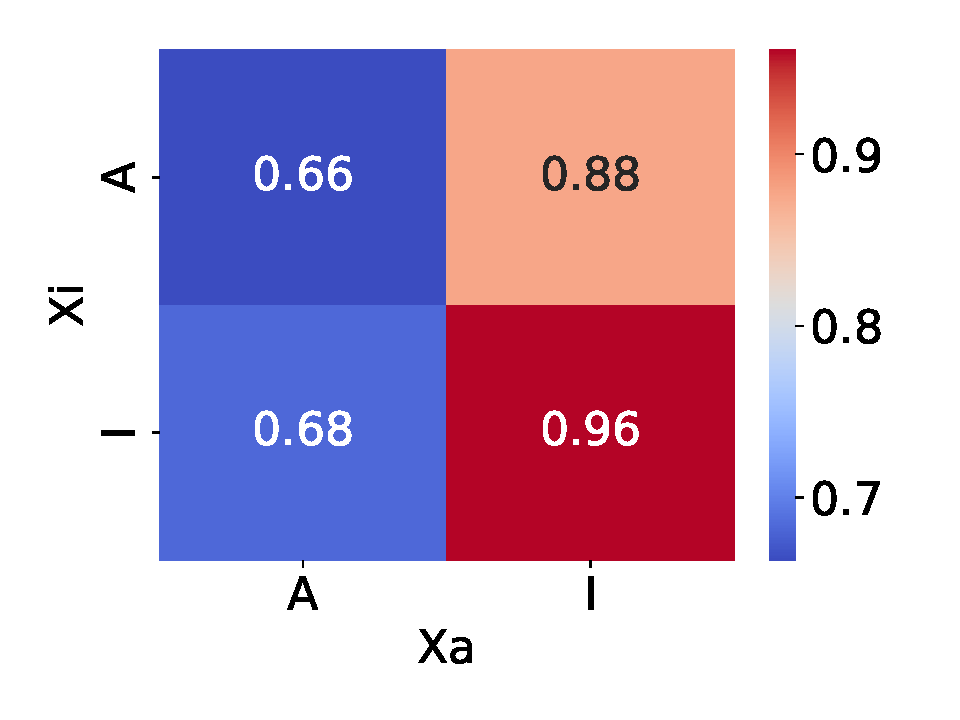
\includegraphics[width=\textwidth]{vary_cross-II-iPSC_timeshifted-rsq-hmap}
                            \caption{Full reactivation}
                        \end{subfigure}
                        \pause
                        \begin{subfigure}[b]{0.49\textwidth}
                            \centering
                            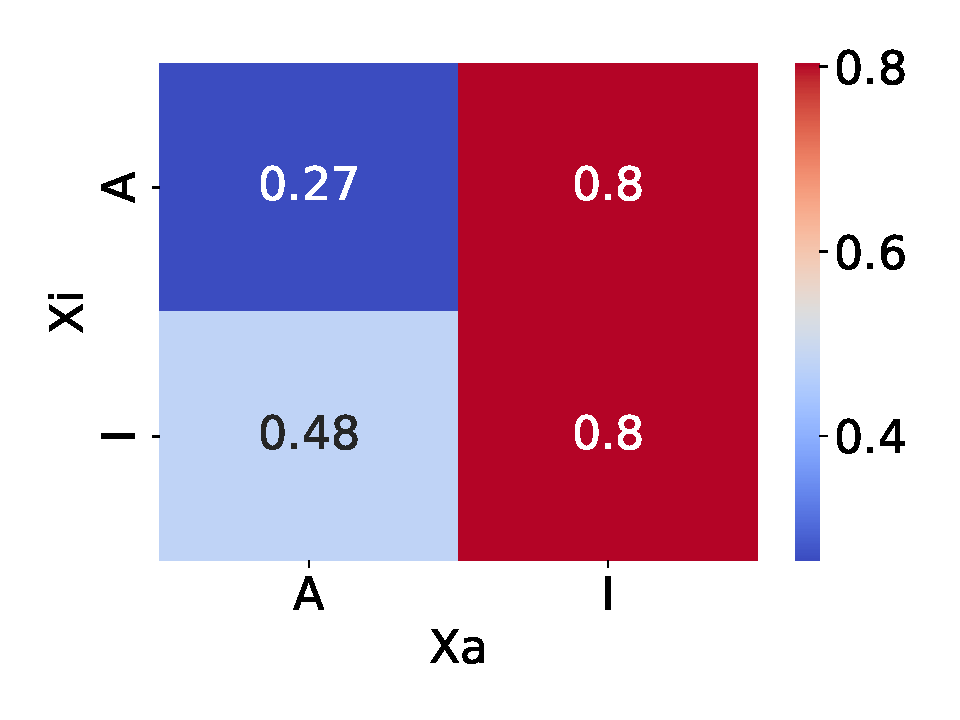
\includegraphics[width=\textwidth]{vary_cross-II-Partial_timeshifted-rsq-hmap}
                            \caption{Partial reactivation}
                        \end{subfigure}
                    \pause[2]\caption{Heatmaps of $R^2$ values}
                \end{figure}
            \end{column}
        \end{columns}
    \end{frame}

    \begin{frame}{Testing cross connections w/ fixed self-activation}
        \begin{columns}
            \begin{column}{0.3\textwidth}
                \begin{figure}
                    \centering
                    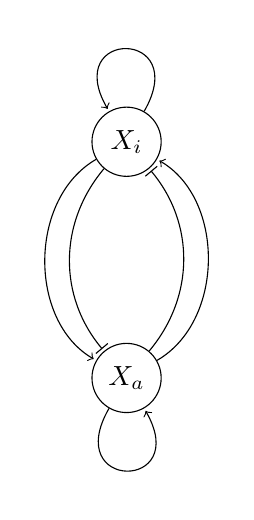
\begin{tikzpicture}[shorten >=1pt,node distance=3cm,on grid,auto]
                        \node[state] (Xi)  {$X_i$};
                        \node[state] (Xa) [below of=Xi] {$X_a$};
                        \path[->]
                            (Xi) edge [out=60,in=120,looseness=7] node {}    (Xi)
                            edge [out=210,in=-210]  node {}    (Xa)
                            (Xa) edge [out=-120,in=-60,looseness=7] node {}    (Xa)
                            edge [out=30,in=-30]  node {}    (Xi);
                        \path[-|]
                        (Xi) edge [out=230,in=-230]  node {}    (Xa)
                        (Xa) edge [out=50,in=-50]  node {}    (Xi);
                    \end{tikzpicture}
                    \caption{Cross connections}
                \end{figure}
            \end{column}
            \pause
            \begin{column}{0.62\textwidth}
                \begin{figure}[h]
                        \centering
                        \begin{subfigure}[b]{0.49\textwidth}
                            \centering
                            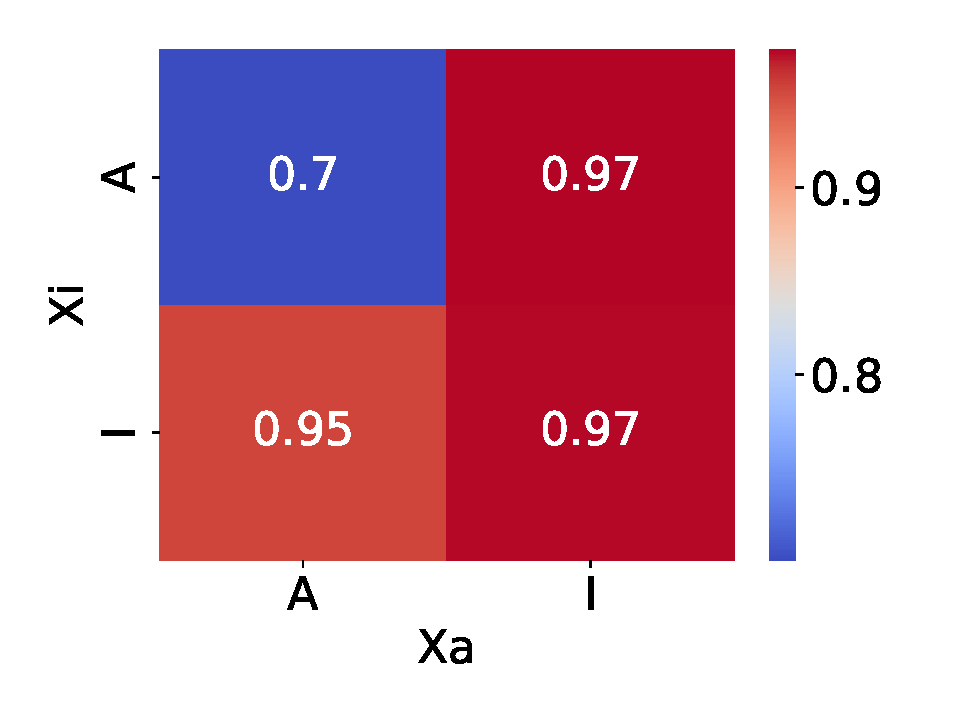
\includegraphics[width=\textwidth]{vary_cross-AA-iPSC_timeshifted-rsq-hmap}
                            \caption{Full reactivation}
                        \end{subfigure}
                        \pause
                        \begin{subfigure}[b]{0.49\textwidth}
                            \centering
                            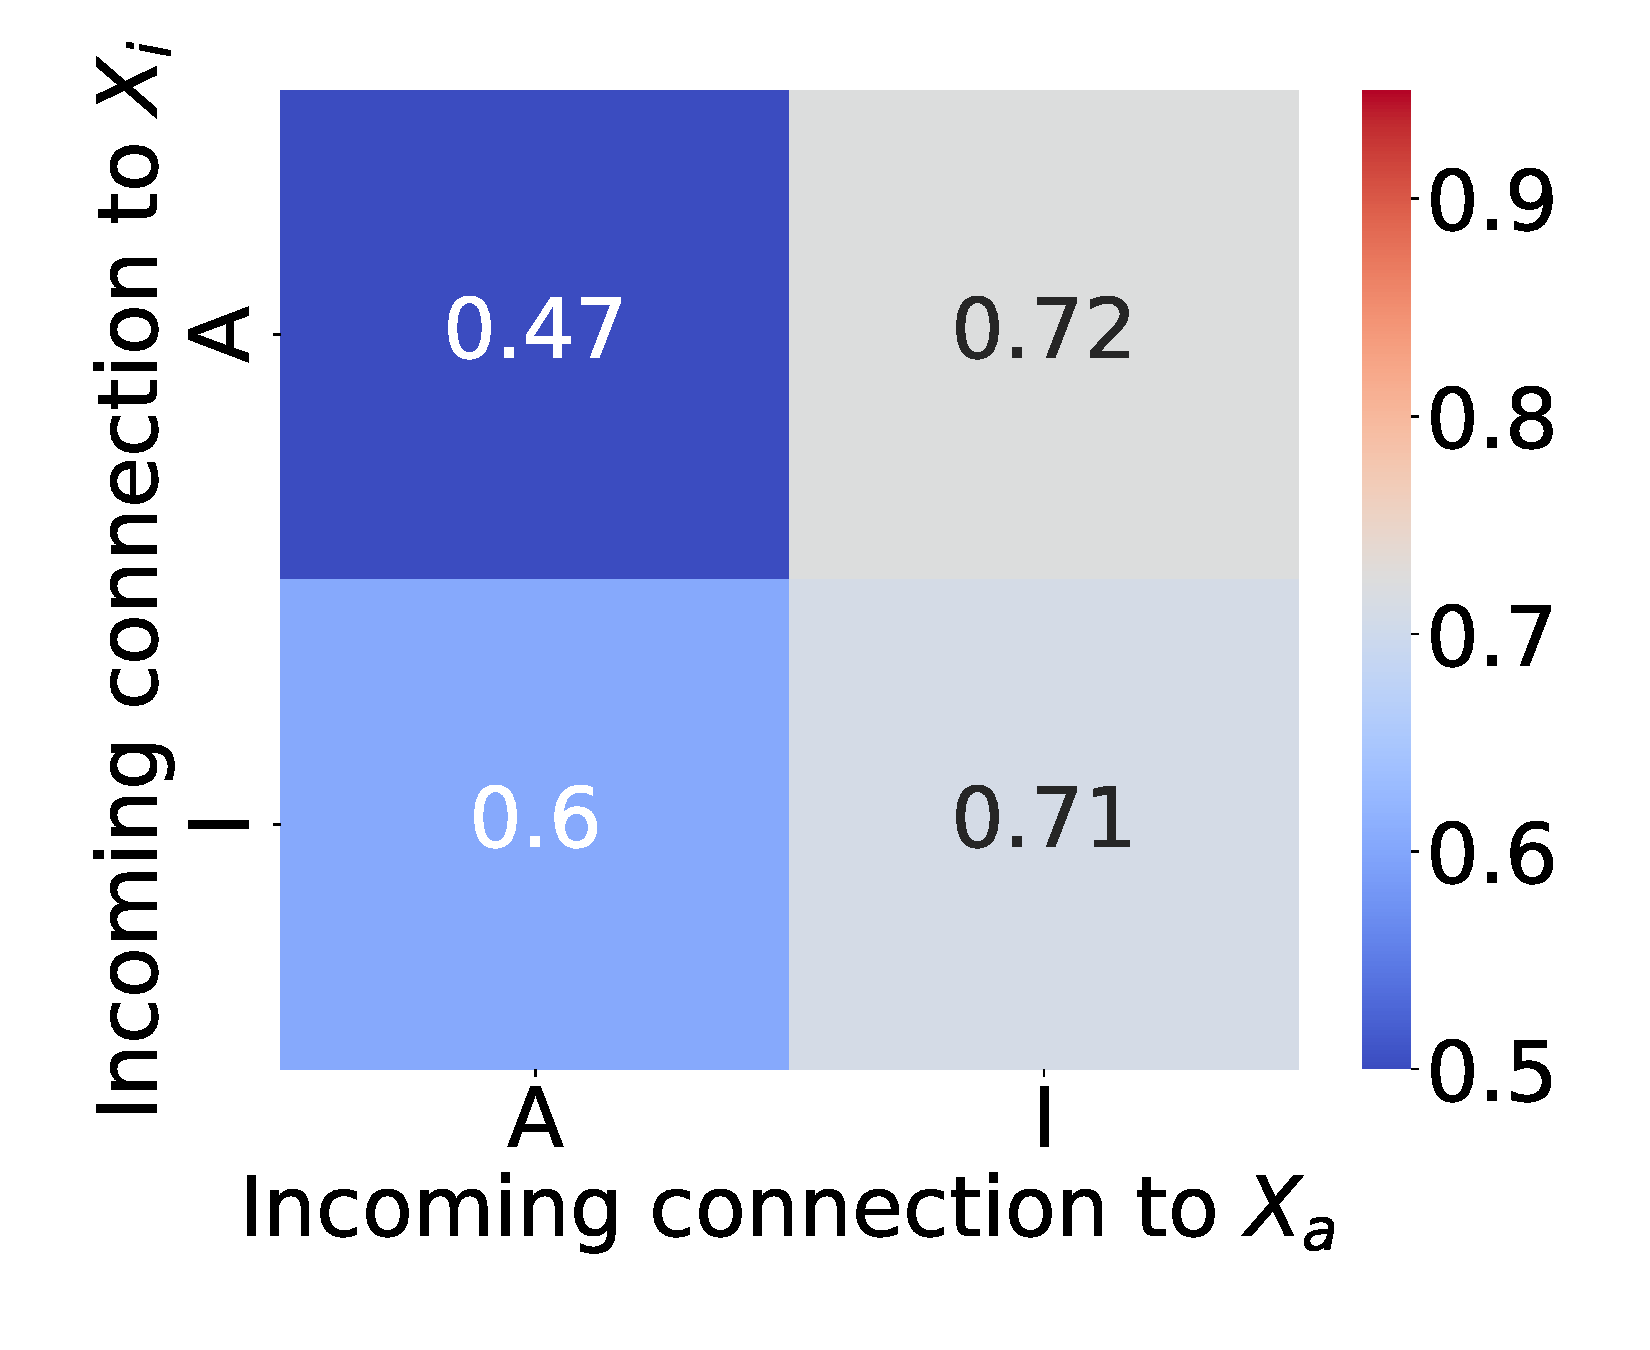
\includegraphics[width=\textwidth]{vary_cross-AA-Partial_timeshifted-rsq-hmap}
                            \caption{Partial reactivation}
                        \end{subfigure}
                    \pause[2]\caption{Heatmaps of $R^2$ values}
                \end{figure}
            \end{column}
        \end{columns}
    \end{frame}

    \begin{frame}{Universal set}
        \begin{figure}[h]
            \centering
            \begin{subfigure}[b]{0.49\textwidth}
                \centering
                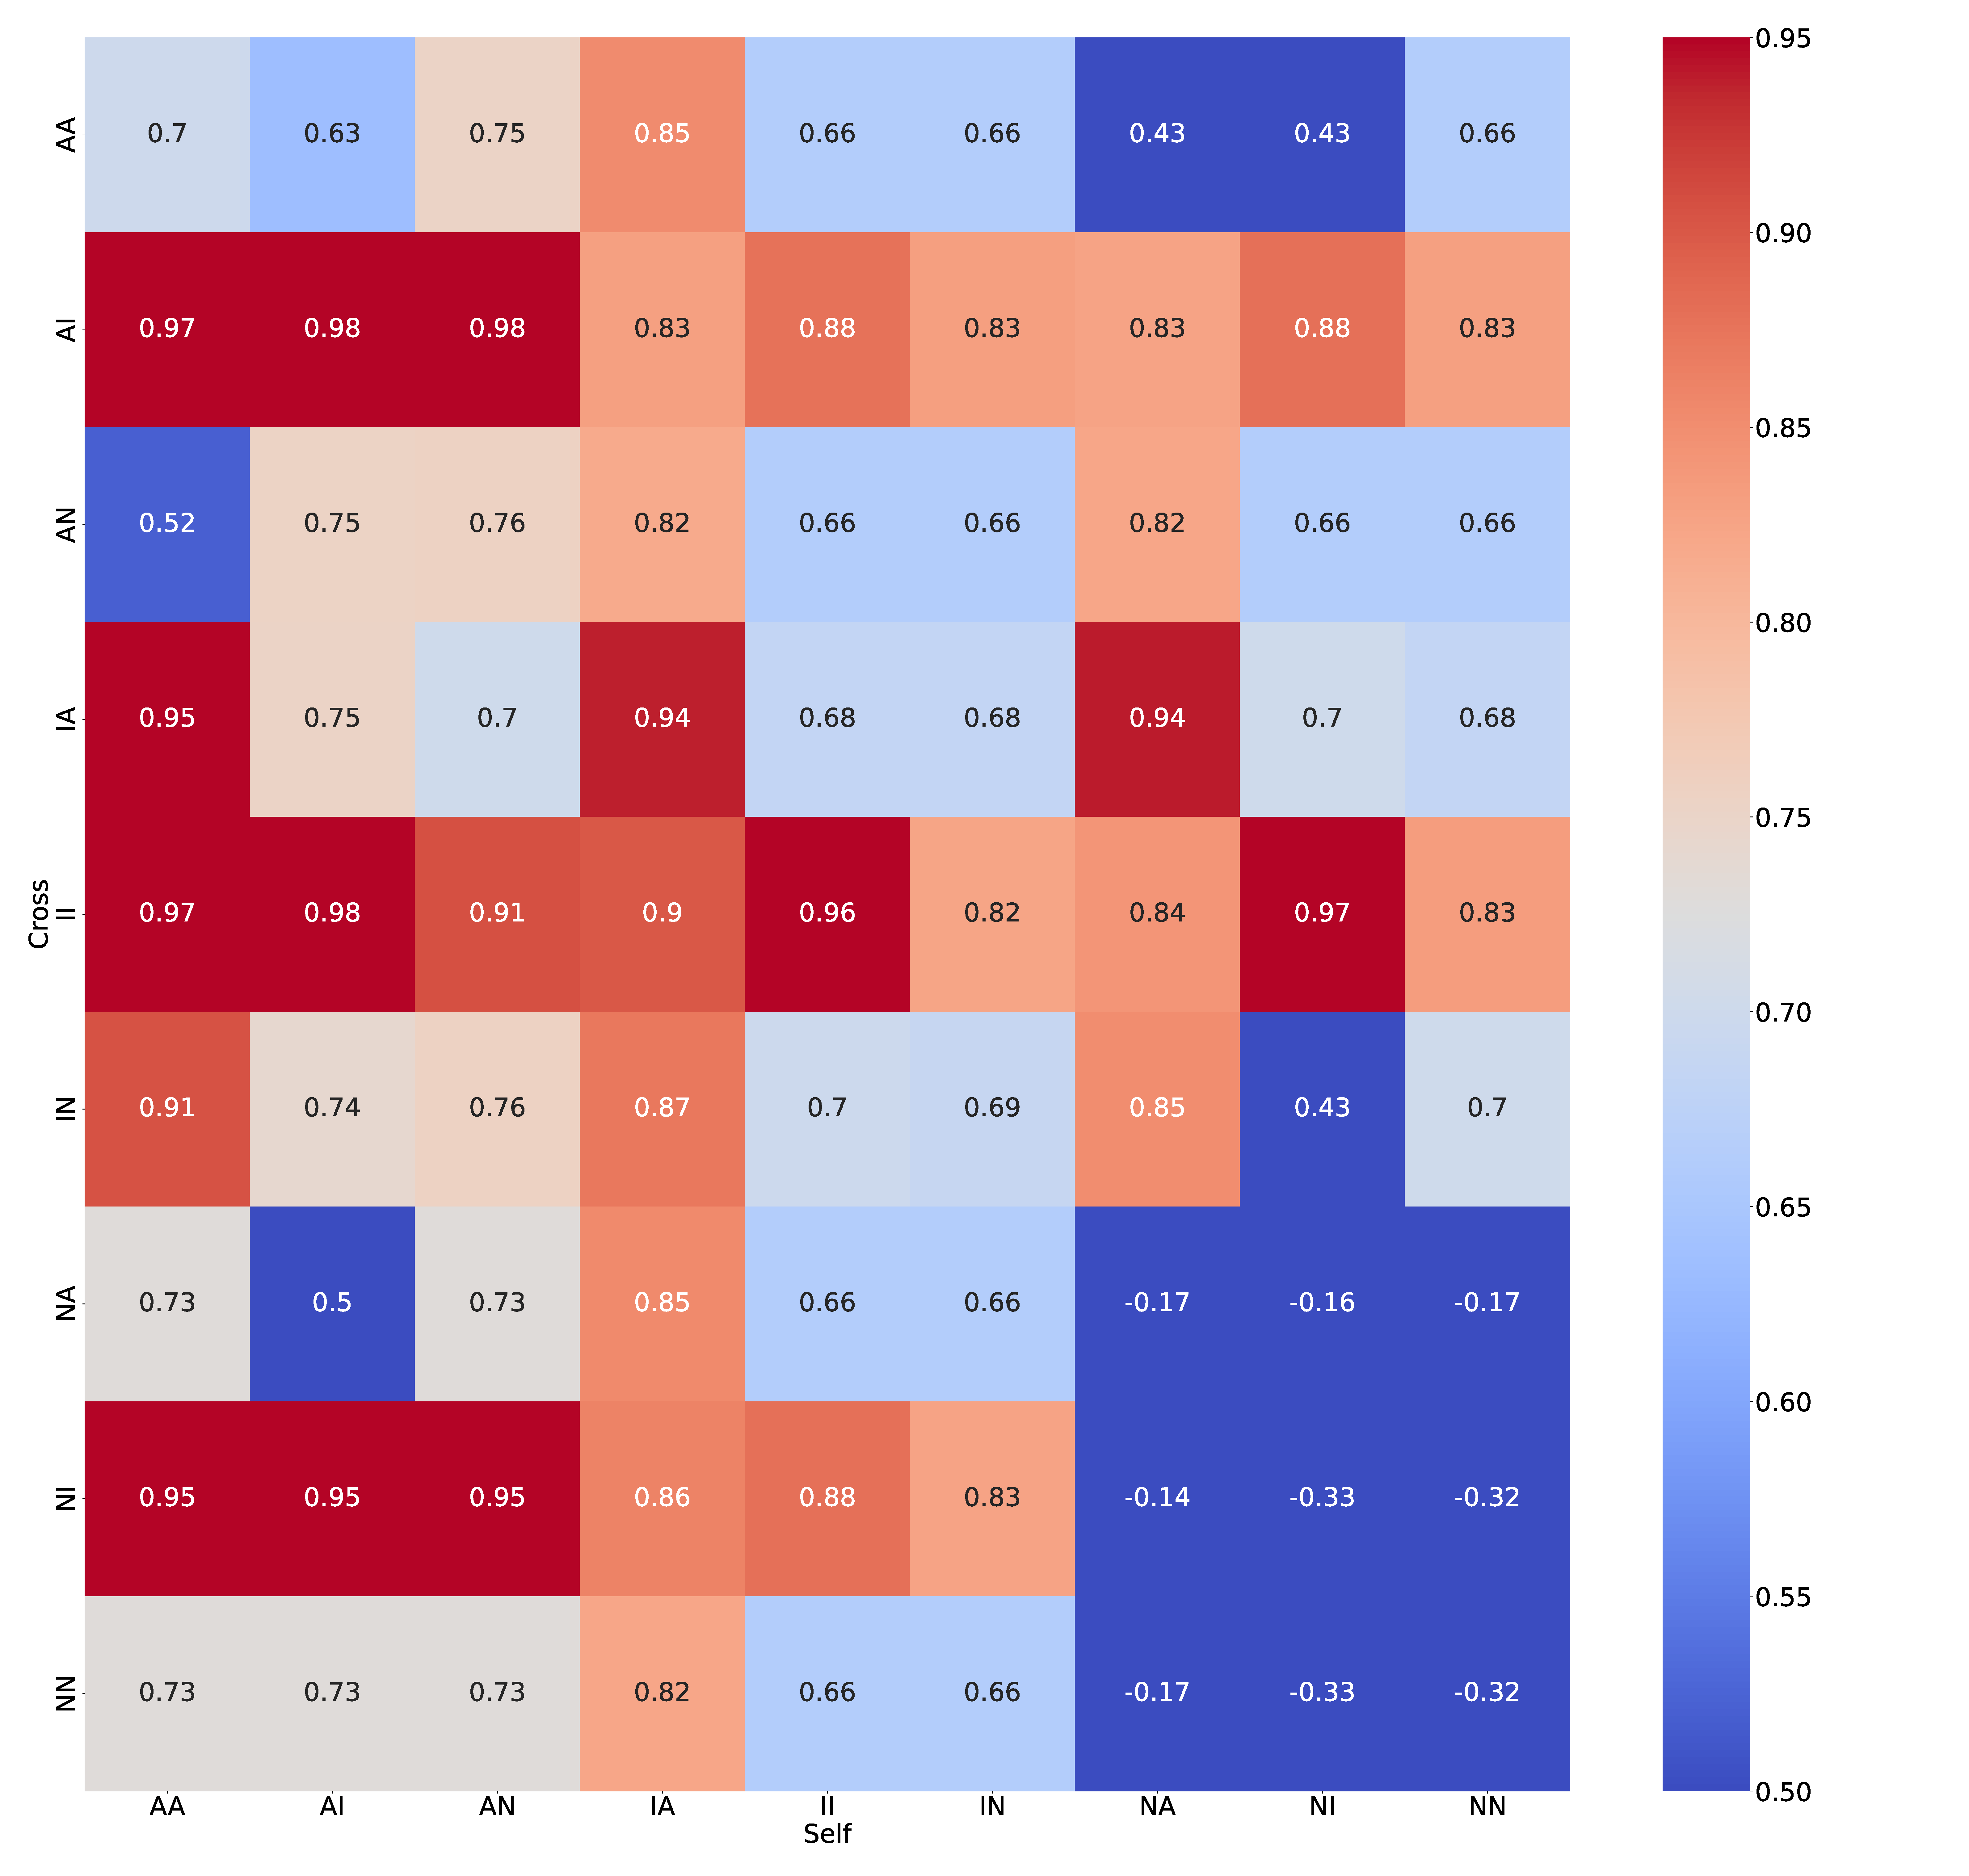
\includegraphics[width=\textwidth]{vary_all-iPSC_timeshifted-rsq-hmap}
                \caption{Complete reactivation}
            \end{subfigure}
            \begin{subfigure}[b]{0.49\textwidth}
                \centering
                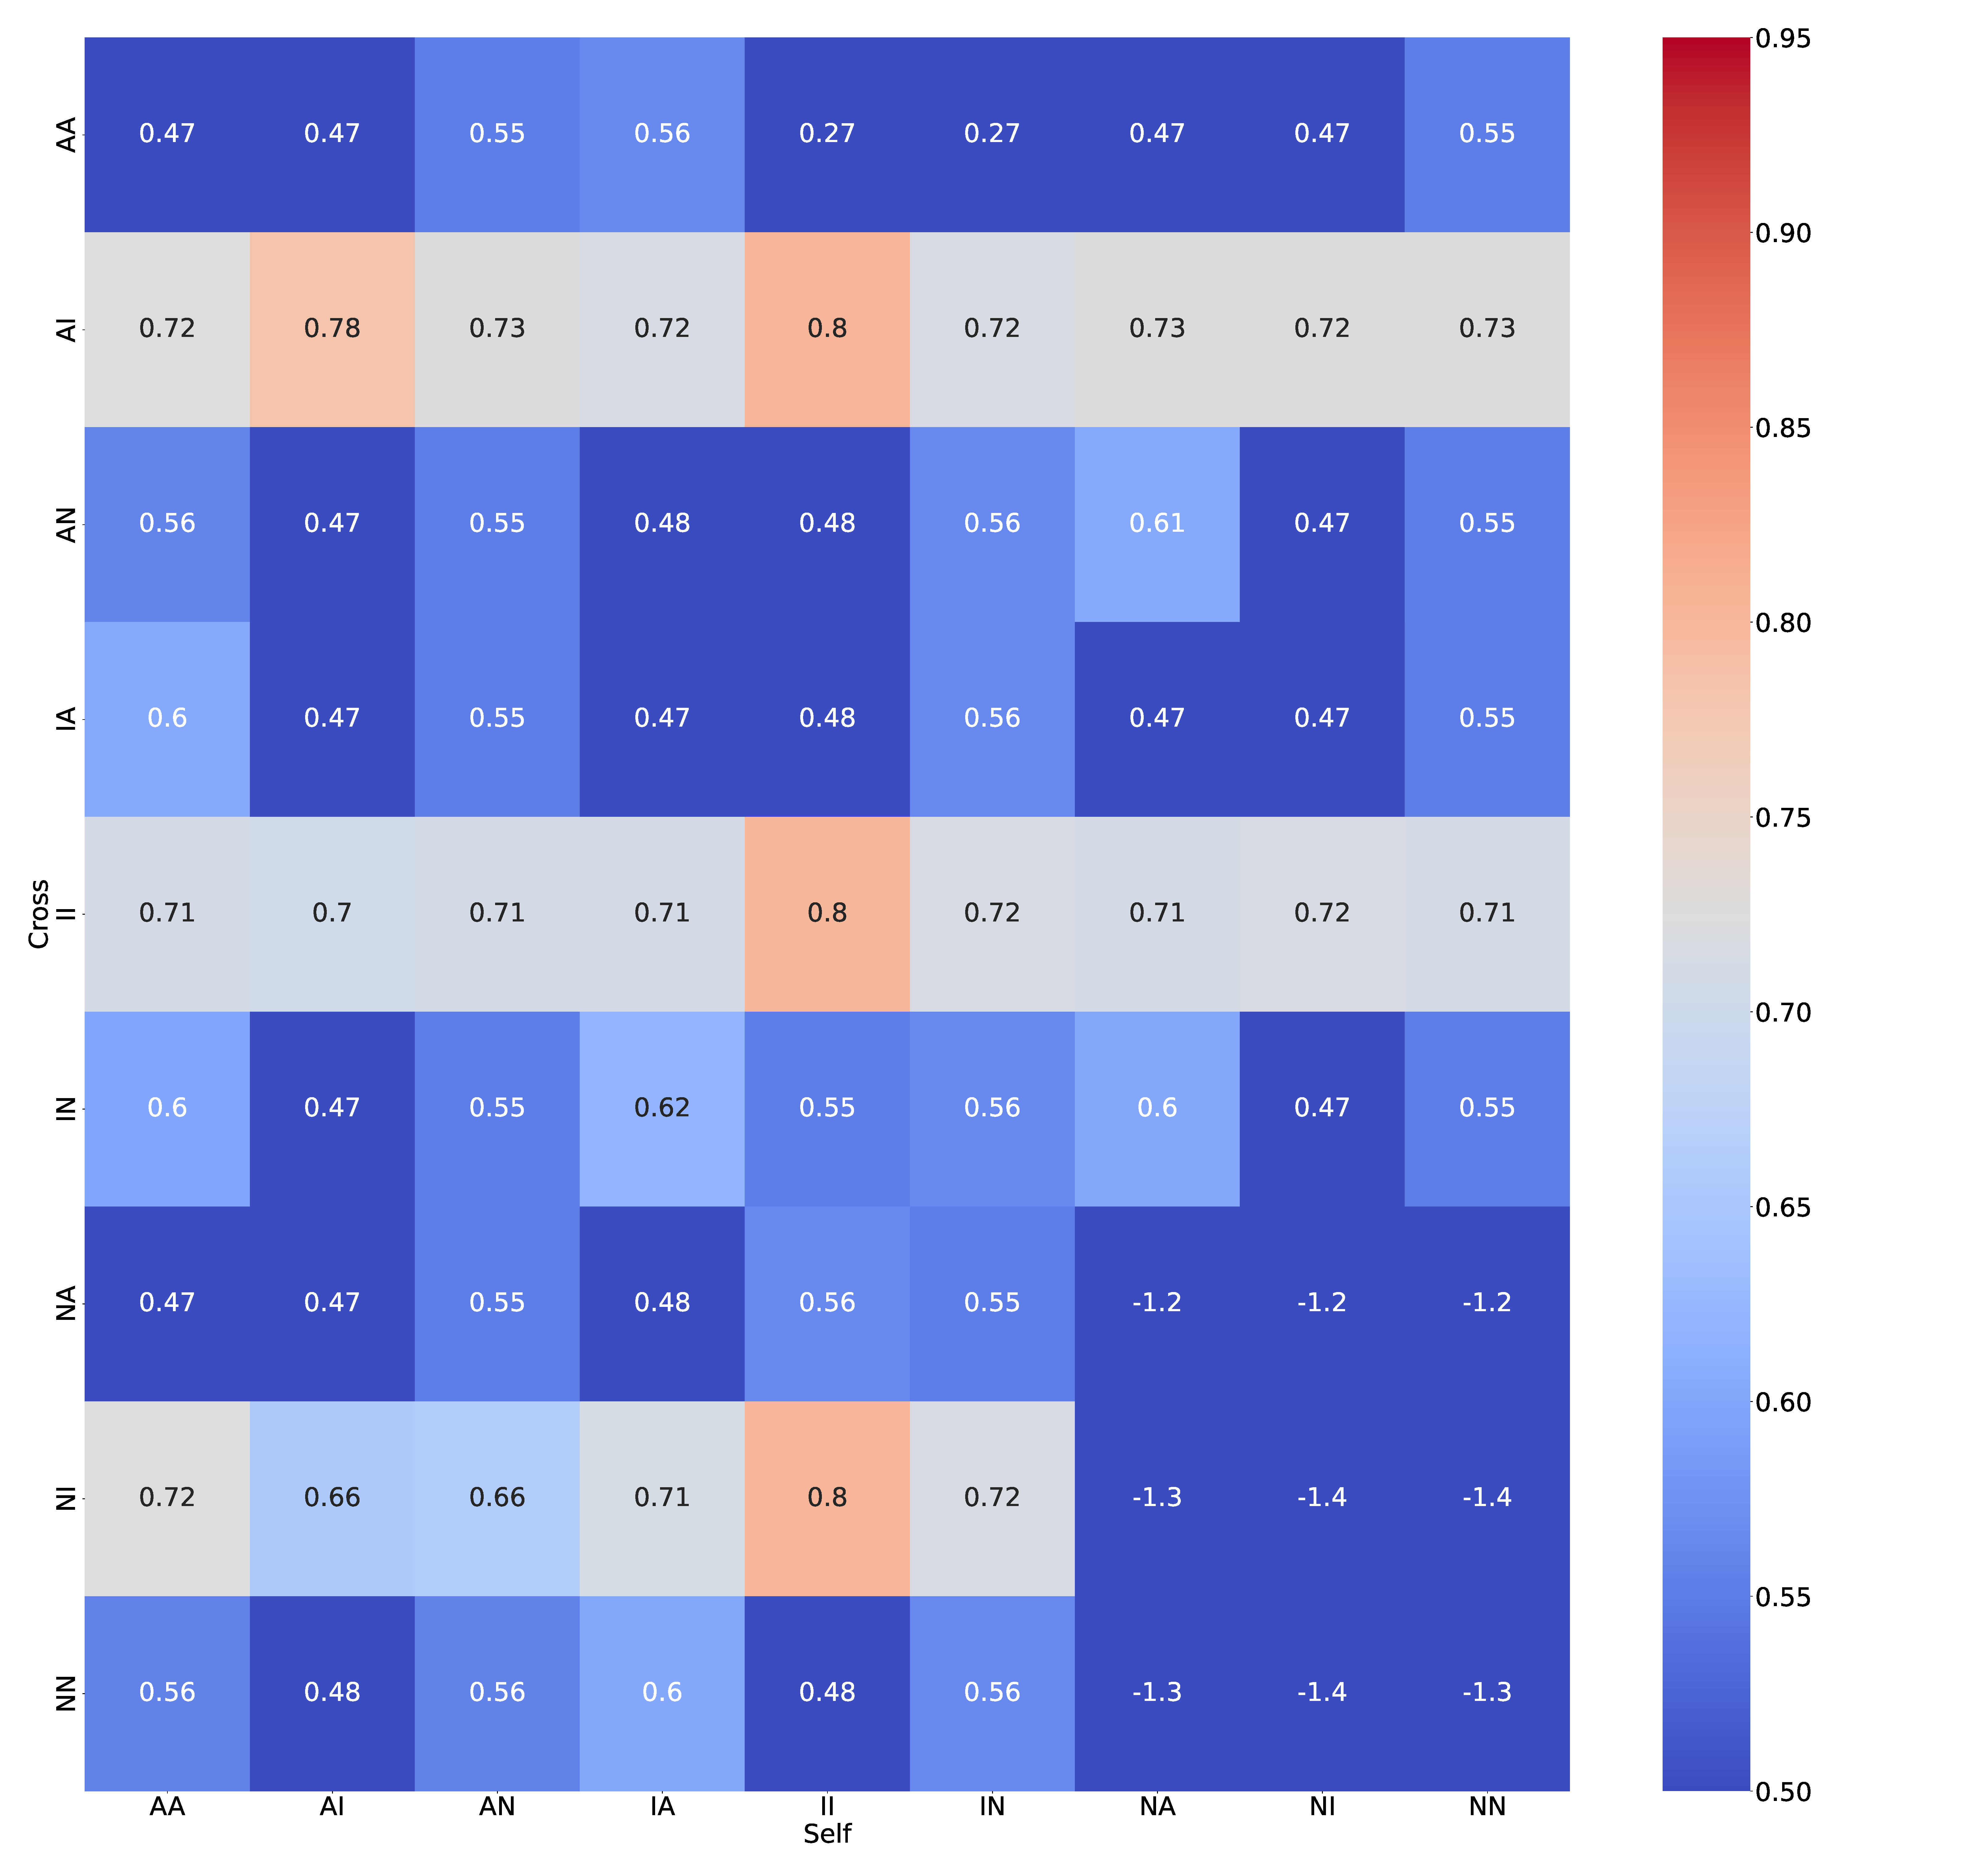
\includegraphics[width=\textwidth]{vary_all-Partial_timeshifted-rsq-hmap}
                \caption{Partial reactivation}
            \end{subfigure}
            \caption{Heatmap of all topologies}
        \end{figure}
    \end{frame}

    \begin{frame}{Complete vs Partial comparison}
        \begin{columns}
            \begin{column}{0.6\textwidth}
                \begin{figure}[h]
                    \centering
                    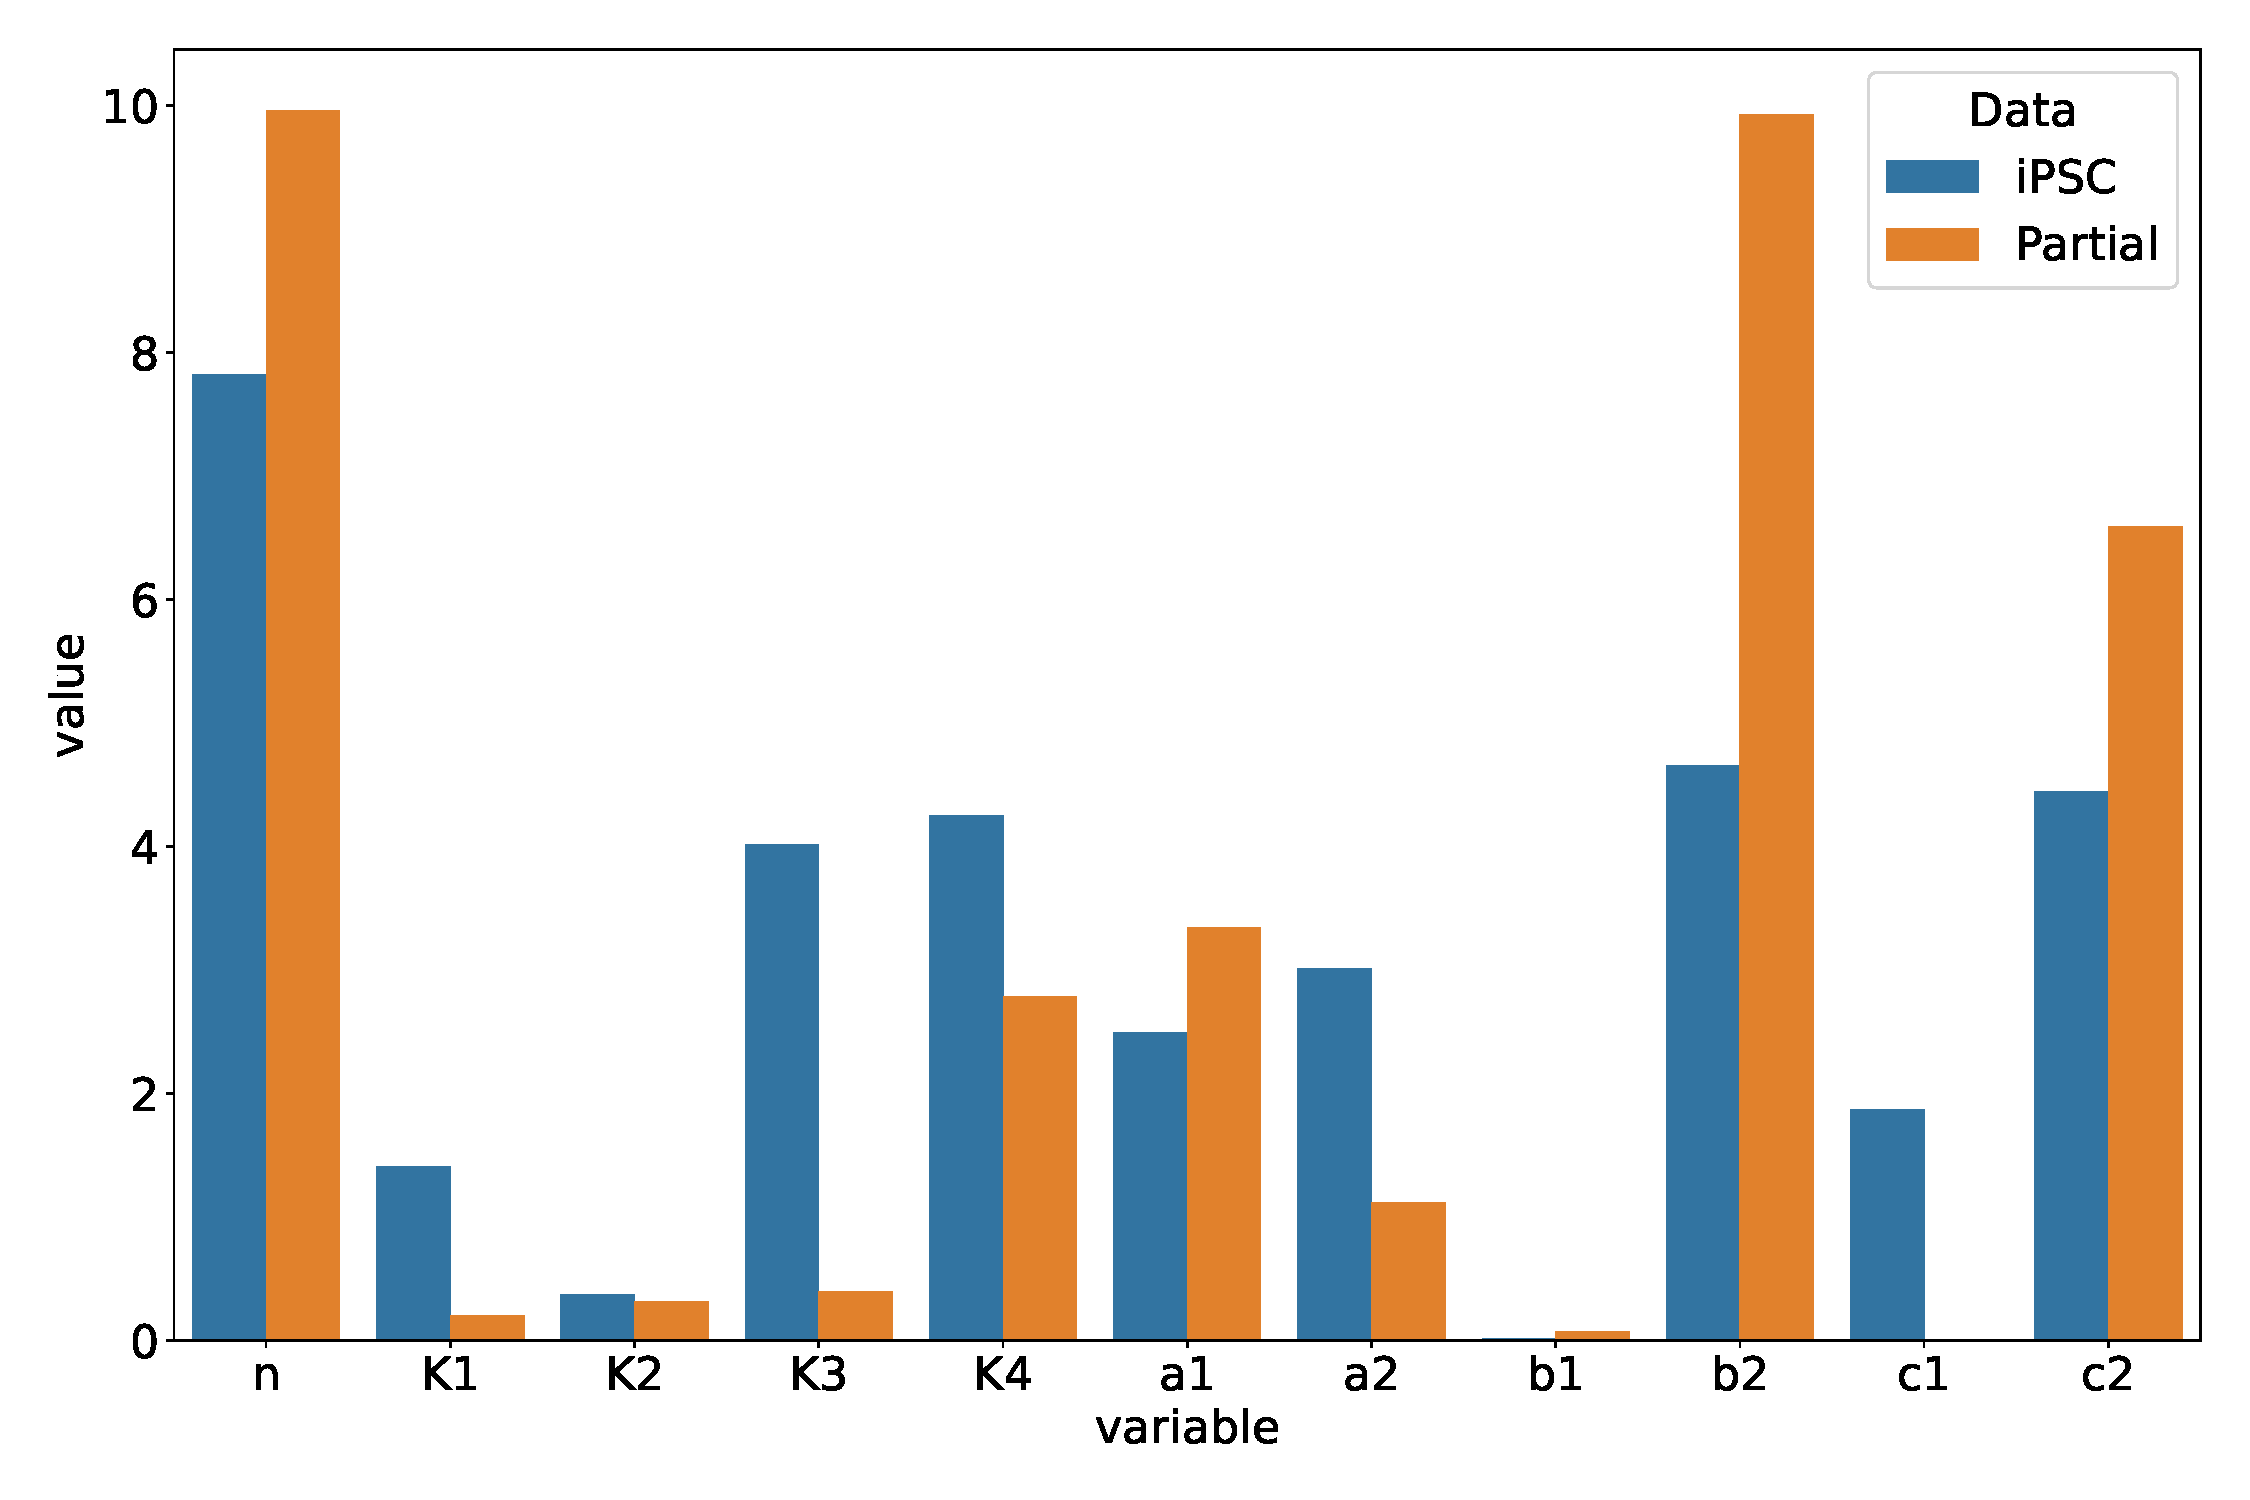
\includegraphics[width=\textwidth]{IIII_timeshifted-parmcomp}
                    \caption{Parameters of fit}
                \end{figure}
            \end{column}
            \begin{column}{0.3\textwidth}
                \begin{itemize}
                    \item cross-inhibition on $X_i$ $\downarrow$
                    \item cross-inhibition on $X_a$ $\uparrow$
                    \item self-inhibition on $X_i$ $\approx 0$
                    \item self-inhibition on $X_a$ $\downarrow$
                \end{itemize}
            \end{column}
        \end{columns}
    \end{frame}

    \begin{frame}{Addition of noise}
        \begin{figure}[h]
            \centering
            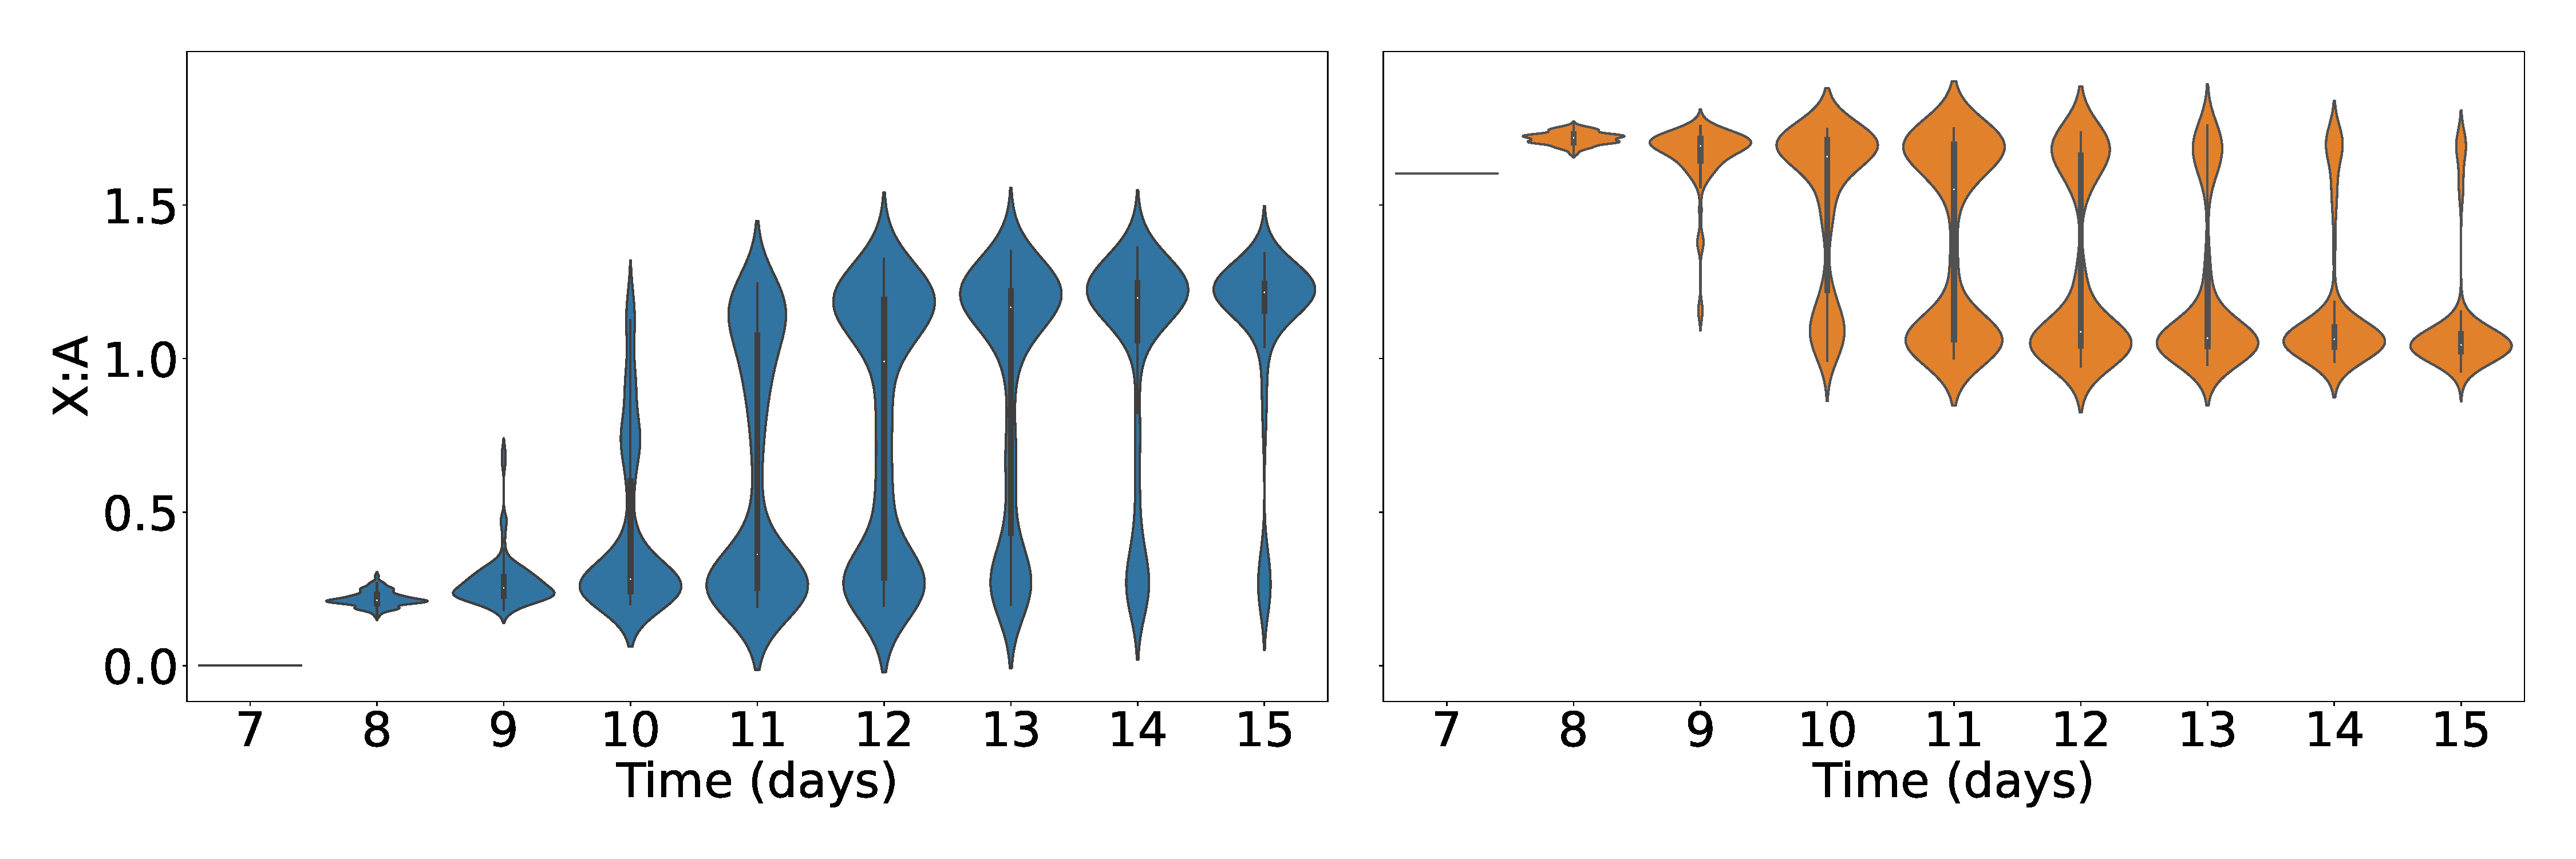
\includegraphics[width=\textwidth]{IIII-iPSC_timeshifted-noise-violin}
            \caption{Reactivation with added noise}
        \end{figure}
    \end{frame}

    \section{Conclusion}

    \begin{frame}{Summary}
        \begin{itemize}
            \item Explains the reactivation dynamics
            \pause \item Explain heterogeneity at timepoint ($X_a,X_i$ vs $X_a,X_r$)
            \pause \item What do these mean?
            \begin{itemize}
                \item Mechanism not fully understood
                \pause \item Competition for factors
                \item Factor mediated interaction
            \end{itemize}
        \end{itemize}
        
    \end{frame}
    
    \begin{frame}{Future plans}
        \begin{itemize}
            \item Time series fits for more complicated topologies with more players?
        \end{itemize}
    \end{frame}

    \begin{frame}[allowframebreaks]
        \printbibliography
    \end{frame}
\end{document}
